\documentclass[a4paper,fleqn,usenatbib]{mnras}
%\usepackage{newtxtext,newtxmath}
\usepackage[T1]{fontenc}
\usepackage{ae,aecompl}
\usepackage{graphicx}	% Including figure files
\usepackage{amsmath}	% Advanced maths commands
\usepackage{amssymb}	% Extra maths symbols
\usepackage{epstopdf}
\usepackage{hyperref}
\usepackage{tikz}
%\usepackage{pgflots}

\def\grs{{GRS\,1739--278\,}}
\def\swiftx{{\em Swift-XRT\,}}
\def\swiftb{{\em Swift-BAT\,}}
\def\xmm{{\em XMM-Newton\,}}
\def\nustar{{\em NuSTAR\,}}
\def\integral{{\em INTEGRAL\,}}
\def\maxi{{\em MAXI\,}}

\def\ferg{erg~cm$^{-2}$~s$^{-1}$}
\def\arcsec{''}
\def\degr{$^\circ$}
\def\arcmin{'}
\def\iaucirc{{IAU~Circ.}}

\title[Low-frequency QPOs in  \grs]{Study of low-frequency quasi-periodic oscillations in \grs during 2014 outburst}

\author[I. A. Mereminskiy et al.]{
Ilya A. Mereminskiy$^{1}$\thanks{E-mail: i.a.mereminskiy@gmail.com},
Andrey N. Semena$^{1}$,
Sergey D. Bykov$^{1,2}$, \newauthor
\,\,Ekaterina V. Filippova$^{1}$,
Alexander A. Lutovinov$^{1}$
\\
% List of institutions
$^{1}$Space Research Institute, Russian Academy of Sciences, Moscow, Russia\\
%$^{2}$Max-Planck Institute for Astrophysics, Garching bei Muenchen, Germany\\
$^{2}$Bauman Moscow State Technical University, Moscow, Russia\\
}


\date{Accepted XXX. Received YYY; in original form ZZZ}

\pubyear{2017}

\begin{document}
\label{firstpage}
\pagerange{\pageref{firstpage}--\pageref{lastpage}}
\maketitle

\begin{abstract}
We detected a type-C low-frequency QPO at 0.3--0.7 Hz in \nustar\, and \swiftx\, data of the black hole candidate \grs\, in the hard-intermediate state during its 2014 outburst, and type-B QPO in the 1.7--5.2~Hz range in the soft-intermediate state. We traced an evolution of spectral-timing properties of the source during the \nustar\, observation. 
As QPO frequency increases, the source spectrum becomes softer, with increasing power-law index and decreasing cut-off energy.

We performed an extended analysis of a rapid X-ray variability. In the power spectrum a prominent QPO and its second harmonic are clearly seen. 
The fluxes in soft and hard X-ray bands are coherent, however the coherence drops with the separation of the energy bands. 
Phase-lags are generally positive (hard) in the 0.1--3~Hz frequency range, and negative below 0.1~Hz.


The accretion disk inner radius estimated with the relativistic reflection spectral model appears to be $R_{\rm in} < 5R_{\rm g}$.
In the frame of the relativistic precession model, in order to satisfy both the observed QPO frequency and derived accretion disk truncation radius a massive black hole ($M_{\rm BH} > 30M_\odot$) is required.
\end{abstract}

\begin{keywords}
X-rays: individual (\grs) -- X-rays: binaries -- accretion, accretion disks  -- stars: black holes
\end{keywords}


\section{Introduction}
\label{sec:intro} 
A study of X-ray variability in accreting astrophysical sources provides a broad view on processes that take a place in such systems. 
This is true both on long (days and weeks), when one speaks about state changes through outbursts of transients sources \citep[see e.g.][]{homan05, heil15}, and on short timescales (down to milliseconds), when the subject under consideration are a quasi-periodic oscillations (QPOs) and broad band stochastic noise. 
A simultaneous usage of spectral and timing data can help to better constrain a geometry of accretion flows around compact objects and infer on processes, which are responsible for generation of the observed spectral-timing features in a self-consistent way.

Some aspects of the spectro-timing evolution of X-ray transients (usually black-hole candidates, BHC) during outbursts can be explained in the frame of the two-temperature accretion flow model \citep{1975ApJ...199L.153E, 1976ApJ...204..187S, 1995ApJ...452..710N}. In this model the accretion flow in the system consists of a geometrically thin cold disk and geometrically thick hot flow (corona). 
It is strongly suggested from observations that this geometrically thick hot flow is responsible for production of a strong variability. 
In particular, using a frequency-resolved spectroscopy \citet{2001MNRAS.321..759C} showed that the variable part of the emission from the BHC system Cyg X-1 has a hard power-law spectrum. 
This spectrum is produced by the Comptonization of soft photons onto hot electrons in the corona, while a stable part of the emission has a cold classical $\alpha$-disc spectrum \citep{shakura73}.  
It is also well known that the total power variability of BHC and neutron star binaries is greater in the hard state (when the spectrum is dominated by the emission produced in the hot flow) than in the soft stsate (when the spectrum can be described with the optically thick $\alpha$-disk model) \citep[][e.t.c.]{1992ApJ...391L..21M, 2000A&A...363.1013R, 2001ApJS..132..377H, 2001MNRAS.321..759C}. 
\citet{1997MNRAS.292..679L} proposed that the observed strong variability (seen as a broad band noise in power spectra) is produced by the stochastic variations of the angular momentum transport efficiency. 
In this propagating fluctuation model a broad band noise of the luminosity is a product of the noise signals from different radii of the accretion flow, owing their characteristic time-scales \citep[see, e.g.,][]{2006MNRAS.367..801A, 2013MNRAS.434.1476I}. 
Therefore, the spectral shape of the broad band noise is determined by the physical and geometrical properties of the accretion flow. In particular, in these papers it was suggested that the broad noise dumping frequency is connected with the inner edge of the accretion flow. 

Another feature, frequently observed in the power spectra of X-ray binaries is different types of QPOs, manifesting itself as a narrow Lorentzian components. 
The low frequency (LF) QPOs are better studied, since they occur at moderate frequencies of 0.1..10 Hz. 
These QPOs are ubiquitous: they were found in systems with neutron stars and black holes \citep{wijnands99}, cataclysmic variables \citep{mauche02} and active galactic nuclei \citep{gierlinskiy08}. 
Few types of LF QPOs are distinguished, based on the shape of power spectra \citep[see, e.g.][]{casella05}, but their origin remains still unclear.


So-called type-C LF QPOs are typically found in X-ray black hole transients during an initial rising part of an outburst and transition to the disk dominated state, i.e. in low-hard state (LHS) and in hard intermediate state (HIMS), according to standard scheme \citep{tanaka96,grebenev97, remillard06, belloni10}, although they are sometimes seen at higher frequencies ($\approx$30~Hz) after transition to high soft state (HSS). 
These QPOs are easy to detect and study, since they are prominent, with $rms\approx10\%$ \citep{casella05}. 
Different authors prescribe a generation of these QPOs to various processes: the Lense-Thirring precession of inner parts of the accretion disk \citep{stella98, ingram09}, oscillations of a standing shock \citep{molteni96}, the accretion rate modulation caused by different phenomena \citep{tagger99,cabanac10} etc. 
In some models, particularly in relativistic precession models (RPM), an observed frequency is strongly dependent on the inner radius of the accretion disk, at which it transforms into a geometrically thick optically thin hot flow. 

Recent advances in simulations of the reflected emission \citep{ross05,garcia14}, arising due to the scattering and absorption of the hard photons in the cold accretion disk, led to the possibility to study a geometry of the disk.  
For such a study to be made it is essential to obtain a broadband X-ray spectrum with high energy resolution - the reflected emission manifests itself by a presence of a prominent, wide and asymmetric iron $K_{\alpha}$ fluorescent emission line at 6.4 keV and Compton-hump at 20-30 keV. 
Adding an information from the X-ray timing analysis one can, in principle, to constrain the location of the component, responsible for the variability, which is though to be a corona or a jet base.
This task presents a challenge, that can be solved only by instruments that posses both a possibility to measure a broadband spectrum with good resolution and corresponding timing capabilities. 
\nustar\, \citep{harrison13_nust}, launched in 2013, is the best available instrument for such studies. 
\xmm and {\it NICER} can be used also, although their energy range reaching only up to $\sim$12~keV limits their capabilities to measure hard tails and the Compton-hump contribution.
Nevertheless there are some great results obtained with these instruments, e.g. the measurement of the Fe K$\alpha$ line profile variation with the QPO phase by \citet[][]{ingram16}. 

In this article we report on first detection of type-C QPOs in HIMS of the Galactic black-hole candidate \grs\, and present a detailed study of properties of the X-ray variability, along with the spectral evolution with \nustar\ and \swiftx instruments.

\section{GRS 1739-278}

\grs is a typical X-ray nova, discovered during an outburst in 1996 \citep{paul96} by the {\it SIGMA} \citep{paul91} telescope onboard {\it GRANAT} space observatory.
Using {\it ROSAT} measurement of the absorption column \citet{greiner96} inferred a distance of 6--8.5~kpc from the estimated absorption, indicating that the source may belong to the Galactic bulge. 
It should be noted that \citet{greiner96} used an X-ray halo size to assess an obscuration column density, and the mean extinction per parsec value from \citet{1973asqu.book.....A} to estimate the distance to the source. 
While this $N_{\rm H}$ estimation appears to be quite precise it is larger than the new measurements of the line of sight absorption in the Galaxy towards the source \citep{1990ARA&A..28..215D, 2005A&A...440..775K, 2006A&A...453..635M, 2014A&A...566A.120S}. 
It means that the source has either an intrinsic obscuration or an additional line of sight obscuration,  and its distance can not be constrained from $N_{\rm H}$.
Nevertheless in this work we will assume that the distance to \grs\ is 8~kpc, given that the source is projected on to the Galactic Bulge.  

Optical and radio emissions were detected during the course of outburst \citep{hjellming96,marti97}. 
\citet{borozdin98} found a strong spectral evolution throughout the outburst to be consistent with the canonical model - the outburst starts from LHS, then soft emission, associated with the optically thick disk starts to dominate, heralding a transition to the high soft state. 
Eventually, they observed very high state and detected a QPO at 5 Hz using {\it RXTE} data \citep{borozdin00, 2001MNRAS.328..451W}.

After 18 years of quiescence \grs\ demonstrated another big outburst, rise of which was detected by \swiftb \citep{krimm14_atel} along with \integral \citep{filippova14}. 
During this outburst an extensive observing campaign by the \swiftx\, telescope was carried out, along with a single long \nustar\ observation. 
After this outburst the source remains active with repetitive mini-outbursts \citep{mereminskiy17grs,yan17}.



\begin{figure*}
\centerline{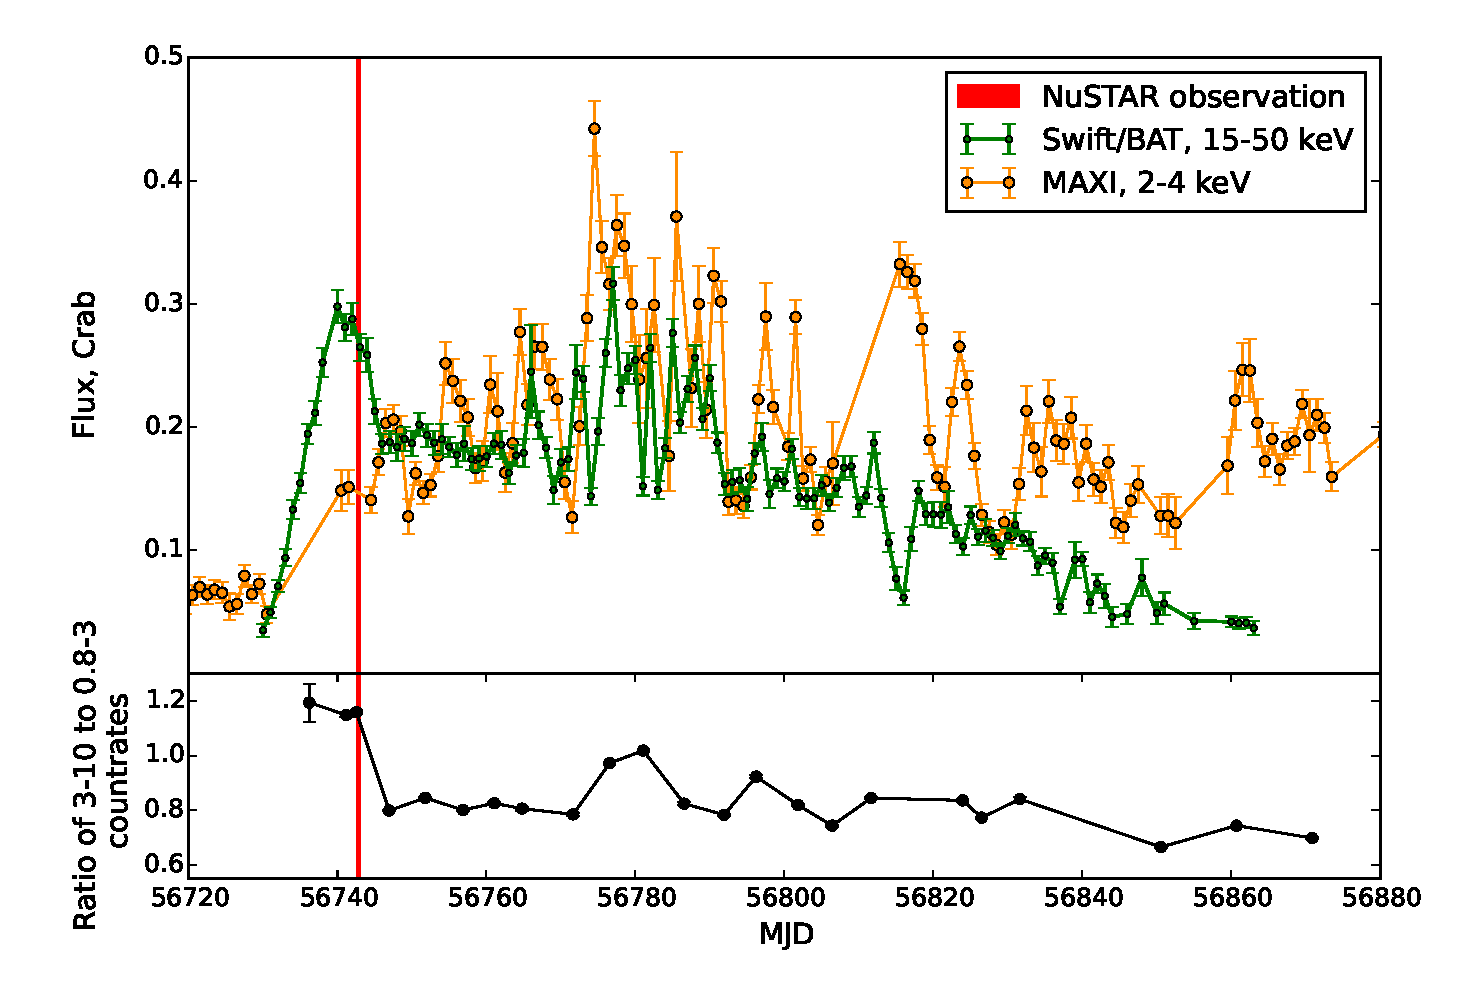
\includegraphics[scale=0.5]{batlc_v06.eps}}
\caption{{\it Upper panel:} green points denote \swiftb\, lightcurve of the 2014 outburst in the 15--50~keV range; orange circles correspond to \maxi\, fluxes in the 2--4 keV energy band.  
Red line shows the time interval of the \nustar\, observation. 
{\it Bottom panel:} evolution of the source spectral hardness during the outburst.} 
\label{fig:batlc}
\end{figure*} 

\section{Observations and data reduction}
\label{sec:datared} 
In order to characterize the overall outburst profile we used data of the \swiftb\, transient monitor \citep{krimm13bat} in hard X-rays (15--50 keV) as well as a soft (2--4 keV) lightcurve from \maxi\, \citep{matsuoka13maxi}.  As a reference value for the Crab we took 0.22 cts cm$^{-2}$ s$^{-1}$ for 15--50 keV band and for 2--4 keV band we took 1.67 cts s$^{-1}$.

We used the \nustar\, observation (ObsID: 80002018002) performed at March 26, 2014 (MJD 56742) and utilized the \texttt{nuproducts} pipeline to extract photons from 2' circular region, centered on the source and to produce lightcurves and spectra.

We also used public observations of \swiftx\, (target ID: 33203) performed regularly over the rise and peak of the outburst.  
Since the source was bright, all \swiftx\, observations were performed in the windowed mode (WT), allowing to study a timing properties of the source. 
We performed a standard analysis with \texttt{xrtpipeline} and barycentered data prior to a lightcurve extraction. 
During several observations countrate was as high as 280 cts s$^{-1}$, therefore we excluded one or few brightest columns depending on the countrate, in order to suppress the effects caused by photon pile-up. 
Photons with energies below 0.8 keV and above 10 keV were filtered out. 
Long-term lightcurves and spectra were obtained from UK Swift Science Data Centre at the University of Leicester \citep{evans09}.

\section{Analysis}
\subsection{Outburst}
A first detection of the source by \swiftb\, occurred at March 9, 2014 (MJD 56725 \citep{krimm14_atel}, we will refer to this date as $\tau_{0}$). 
An outburst profile in hard X-rays (15--50~keV) featured fast rise with a tenfold intensity increase over ten days (see Fig.~\ref{fig:batlc}), nearly flat-top peak ($\tau_{0}$+10..+15 days) followed by an abrupt flux decrease by 30\% over the course of two days.
After this, the source demonstrated a gradual decline interrupted by a flaring activity at $\tau_{0}$+50..+70 days. 
At $\tau_{0} \approx +86$ days a sharp dip occurred in the \swiftb\ lightcurve. 
After the cease of the outburst the source was remained active with flux about 5--15 mCrab. 

An addition of data from \maxi\, to the \swiftb\, lightcurve gives us another insight on the outburst evolution. 
Comparing fluxes in soft and hard bands one can see that the soft component obviously lags hard emission in the beginning of the outburst, but then starts to grow and ends up dominating during the flaring period as well as during the hard dip. 
The bottom panel of Fig.\,\ref{fig:batlc} shows an evolution of the hardness ratio (3--10~keV/0.8--3~keV) measured by \swiftx. 
The detailed analysis of the spectral evolution during the outburst will be presented elsewhere (Bykov et al., in preparation).

Fortunately, the \nustar\ observation triggered by \cite{miller15_nust} was carried out right at the transition between hard and soft states, thus giving us an unique opportunity to study processes that happens during the hard-intermediate state. 


\subsection{NuSTAR observation}
\label{sec:nust} 

\nustar\, observed \grs\ for nearly 30 ks of the net exposure right after the hard X-ray peak (at $\tau_{0}\approx+18$, Fig.~\ref{fig:batlc}). 
Given the 96.9 minute orbital period of \nustar, the observation is divided in 13 intervals separated by Earth occultations, as shown in Fig.\,\ref{fig:nust_lc}. 
We denoted these intervals with roman numerals, from {\bf I} to {\bf XIII}. 
From the lightcurve it is clear, that the source flux is increased throughout the observation from $\approx$145 up to $\approx$170 counts per second. 
The spectrum is also altered, with the hardness (defined as a ratio of countrates  $R_{3-10\,keV}/R_{10-78\,keV}$) had been growing monotonically from 2.7 to 3.1 (Fig.\,\ref{fig:nust_lc}). 

\subsubsection{Broadband average spectrum}
\label{sec:spec}            

\citet{miller15_nust} shown that the average spectrum during the observation is well described by the relativistic reflection models such as \texttt{reflionx} \citep{ross05} and \texttt{relxill} \citep{garcia14, dauser14,dauser16} with the accretion disk that reaches remarkably close to the black hole innermost stable circular orbit (ISCO). 
The disk inner edge radius was estimated as $R_{\rm in} = 5^{+3}_{-4}\, G M/c^{2}$ \citep{miller15_nust}. 
It was also noted that no additional thermal component was needed to describe the energy spectrum, probably due to the low disk temperature and high absorption.

We would like to mention that the obtained spectrum (Fig.\ref{fig:spec}, see also Fig.2 in \citet{miller15_nust}) has a very complicated shape, that is unlike the canonical LHS \citep{zdziarski04}, when power law extends up to a few hundred keV without cutoff, as was observed in \grs\, during the failed outburst in 2016 \citep{mereminskiy17grs}.

We used a \swiftx\, observation (ObsId: 00033203003, 1.3 ks exposure) that coincides with the \nustar\, observation, to extend the energy range up to 0.8--78 keV, allowing one to search for the thermal emission associated with the cold inner disk with $kT \sim 0.1...0.4$~keV (similar was found in other BHCs, see \cite[][ etc]{miller06b,miller06a,parker15}).

For the spectral fitting we used \texttt{XSPEC} package \citep{arnaud96}.
We applied {\it relxilllp} (v1.0.2) spectral model that describes the reflection of emission, produced by a point source located on the rotation axis above the Kerr black hole, from the relativistic accretion disk. 
We selected this model for several reasons - first, \cite{miller15_nust} found that it matches {\it NuSTAR} data well. 
Also, during the 1996 outburst source was detected at radiowaves, possibly indicating jet activity, the jet foundation are often thought to be responsible for this type of ``lamp-post'' geometry. 

For spectral fitting we used \texttt{migrad} minimizer from {\em MINUIT} package \citep{james75minuit}, and in order to estimate errors we employed a large MCMC chain. 
We extracted \swiftx\, spectrum using only zero-grade events, grouped it to has at least 30 counts per bin and added 3\% systematic error. Similar grouping were applied to \nustar\, data. 

Usage of this spectral model and fixed absorption column ($N_{H} = 2.15\times10^{22}$ cm$^{-2}$, \citep{fuerst16_gx339}) led to fits with systematic negative residuals below few keV. 
Therefore, we left $N_{H}$ free and obtained value of 2.64$\times10^{22}$ cm$^{-2}$. 
No additional soft component is required in order to describe broadband spectra.

It should be noted, that \grs\, is known to demonstrate a large dust scattering halo \citep{greiner96}. 
Similar halo was observed during this observation (K.L. Page, private communication). 
It may introduce some bias in the spectrum normalisation, which is expected to be up to 15\% level. 
Therefore, this discrepancy in measured absorption column densities could be partially caused by the unaccounted halo emission.

Obtained upper limit on the accretion disk truncation radius - $R_{in} < 9 GM/c^{2}$ (90\% confidence limit) is similar to the value from \cite{miller15_nust}, height of the ``lamp'' above the accretion disk is in agreement too (see Tab.~\ref{tab:fullfit} for obtained parameters). 
Some discrepancy seen in the parameters of the accretion disk - e.g. inclination, ionization parameter and Fe-abundance, it can be caused by a broader energy range used in this study. 

Total unabsorbed flux in 0.1--100 keV band is about 1.4$\times$10$^{-8}$~erg s$^{-1}$ cm$^{-2}$ which translates to a luminosity of 1.1$\times$10$^{38}$ erg s$^{-1}$ for the 8 kpc distance. 
Typical luminosity at which BHCs change from LHS to HIMS is about $0.1 L_{Edd} = 1.2\times10^{37} (M/M_{\odot})$ erg s$^{-1}$ \citep{2010MNRAS.403...61D}, although we should note that there is significant scatter in this value. 
Therefore one can put a rough estimate on the black-hole mass as 9 $M_{\odot}$, assuming 8 kpc distance.

\begin{table}
\noindent
\centering
\caption{Best-fit parameters of \texttt{phabs*relxilllp} model}
\label{tab:fullfit}
\centering
\begin{tabular}{|c|c|}
\hline\hline
Parameter & Value \\
\hline
$N_{H}, 10^{22} cm^{-2}$ &   2.64$^{+0.05}_{-0.03}$ \\   
$h, GM/c^{2}$   &  22.3$^{+0.6}_{-4.3}$ \\
$a, cJ/GM^{2}$    & 0.73$^{+0.26}_{-0.23}$   \\
$incl, deg$ & 22.1$^{+2.9}_{-2.0}$ \\
$R_{in}, ISCO$  & 1.05$^{+1.73}_{-0.02}$ \\ 
$\Gamma$& 1.40$^{+0.01}_{-0.01}$   \\
$\log{\xi}$ &  3.52$^{+0.05}_{-0.07}$ \\
$A_{Fe}$   &  3.0$^{+0.6}_{-0.3}$  \\        
$E_{cut}, keV$    &       26.3 $^{+0.3}_{-0.5}$    \\
$R_{refl}$  &         0.42$^{+0.03}_{-0.03}$    \\
$N_{FMPA},\,\times10^{-2}$          &      1.49$^{+0.09}_{-0.03}$ \\
$C_{FMPB}$ & 1.017$^{+0.002}_{-0.001}$    \\
$C_{Swift-XRT}$    &   1.04$^{+0.01}_{-0.01}$\\
$\chi^{2}_{red.}$    &   1.1=\\ 
              &= 3366.21/3062 d.o.f\\
              
\hline
\end{tabular}
\end{table}




\begin{figure}
\centerline{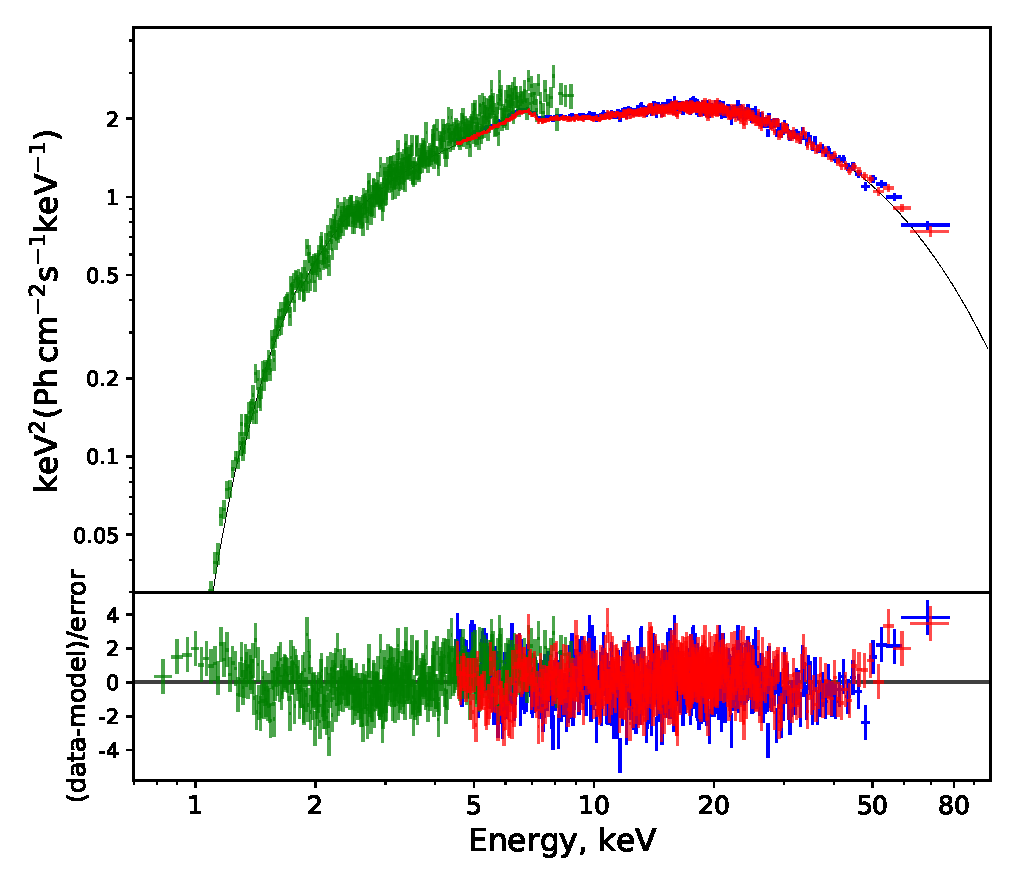
\includegraphics[width=\linewidth]{spectrumfit_v05.pdf}}
\caption{Fit of composite \swiftx/\nustar spectrum by \texttt{phabs*relxilllp} model. Green, red and blue points correspond to \swiftx, \nustar FPMA and FPMB, correspondingly.} 
\label{fig:spec}
\end{figure}  



\subsubsection{Evolution of the continuum and constrains on the movement of the inner parts of the accretion disk}
\label{sec:continuum_evolution}
To get a better view on the evolution of the continuum emission we fitted all individual intervals spectra with the absorbed \texttt{xillver} \citep{garcia13} model (\texttt{const*phabs*xillver}). 
This model describes the reflection of the incident radiation from the ionized slab of the matter. 
The spectrum of the incident radiation is assumed to be a power-law with the exponential cutoff. 
We picked the \texttt{xillver} model over the \texttt{relxilllp} for the analysis of separate intervals because we wanted to describe changes in the continuum emission making no assumptions on the system geometry. 

Spectra from two \nustar\, modules for each interval were fitted simultaneously with free cross-calibration constant between modules.
Before fitting, spectra were grouped in order to have at least 100 counts per bin, channels above 60 keV were ignored, due to the low statistics of high-energy photons. 
Since we used only {\it NuSTAR} data for this analysis we fixed interstellar absorption at $N_{H} = 2.15\times10^{22}$ cm$^{-2}$, as was found by joint \xmm/\nustar\, observation during the low luminosity state \citep{fuerst16}. 
Element abundances were taken from \cite{wilms00} and cross-sections from \cite{verner96}. 
A relative iron abundance was fixed at  $A_{Fe} = 1$, an ionization parameter and an inclination at $\xi=3.2$ and 35 degrees, respectively, in consistency with results of \citet{miller15_nust}, obtained with different spectral models. 
Although in the \texttt{xillver} there is no relativistic broadening of the Fe K$\alpha$ emission line no significant residuals in the 5--8 keV region are seen, mainly because of the limited statistics in per interval spectra. 
Resulting fits are of satisfactory quality with $\chi^{2}/d.o.f. \approx 1.05$. 
 
The examination of the best-fit parameters (see Fig.\ref{fig:intspe}) confirms that the spectrum soften during the observation and the cut-off energy decreases. 

\begin{figure*}
\centerline{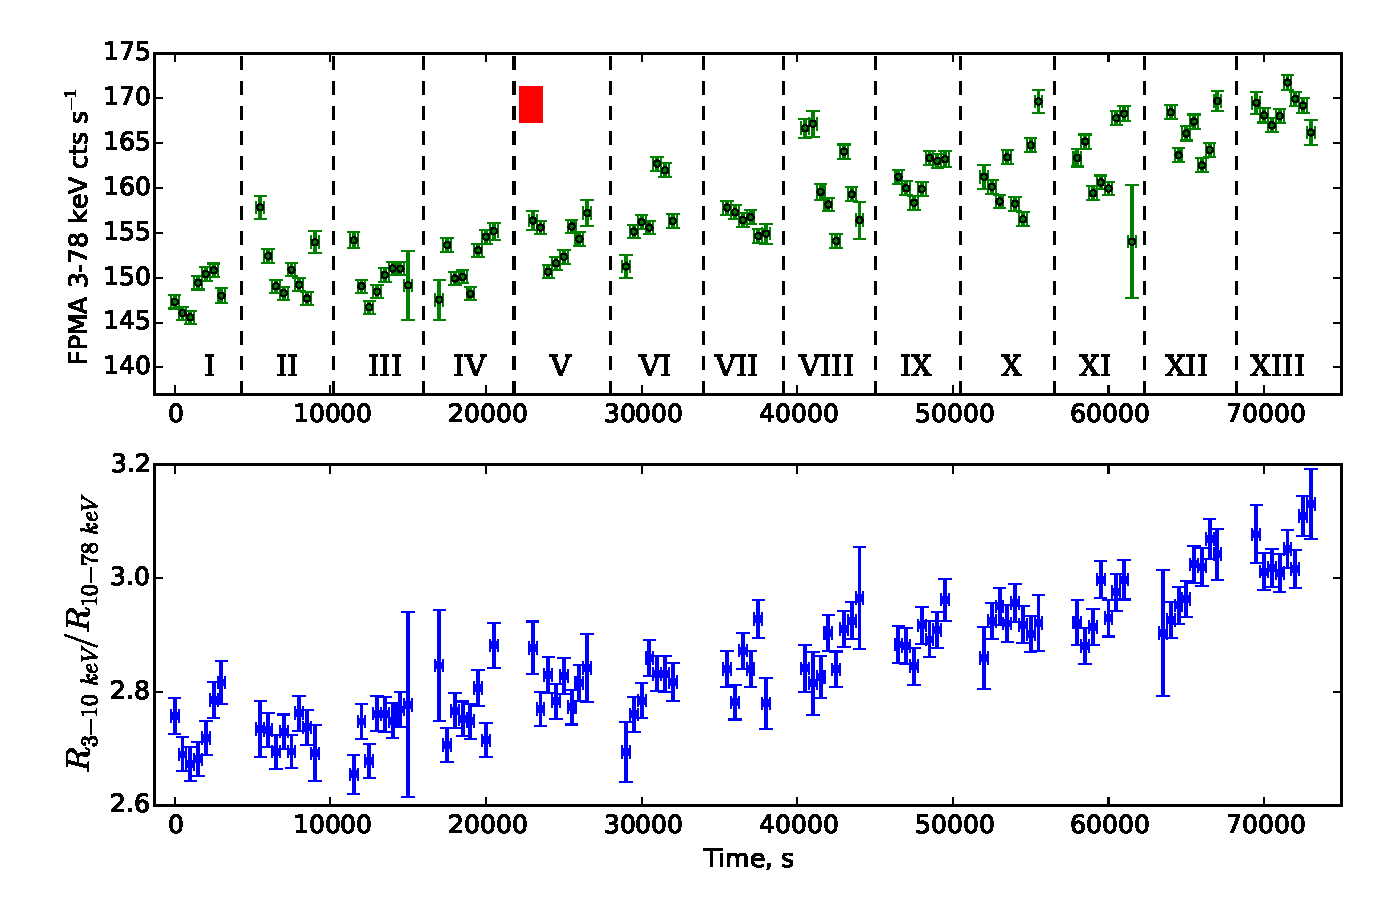
\includegraphics[scale=0.7]{nuAlc_color_v04.eps}}
\caption{Upper panel: countrate of \nustar\,FPMA in 3--78 keV band. We enumerated intervals of uninterrupted observations with roman numerals. Red square shows time of simultaneous \swiftx observation (ObsId: 00033203003, second part). Bottom panel: evolution of hardness during observation} 
\label{fig:nust_lc}
\end{figure*} 

Spectra for single intervals have not enough statistics to constrain changes of the Fe-line profile and, as a sequence, to determine whether the disk inner boundary  is moving during the observation. 
To increase the statistics, we split whole observation into three major parts, with the first one consisting of intervals {\bf I-IV}, the second of {\bf V-IX} and the third of {\bf X-XIII} and extracted spectra in 4--78 keV band. 
We grouped them in order to have at least 100 counts per bin and then fitted them (excluding data between 5--10 keV) with the simple \texttt{phabs*cutoffpl} model, again using $N_{H} = 2.15\times10^{22}$ cm$^{-2}$.  

Plotting the ratio of this fit to initial spectra (Fig.~\ref{fig:ratios}) one can see that two strong features, a broadened Fe-line at 5--9 keV and a Compton hump around 30 keV are stable. 
We estimated the equivalent width of  Fe K$\alpha$ emission line in this three parts - we approximated 4--78~keV spectra with 10--30~keV range being ignored (to neglect the Compton-hump contribution) with model consisting of absorbed cut-off powerlaw and gaussian. 
Equivalent width of the gaussian component is around 0.175 keV and remains constant along the observation within error margins, although it is possible that the quality of data is not enough to trace the real change.
Therefore we can conclude, that there is no drastic change in position of inner disk boundary during the observation. 

\begin{figure}
\centerline{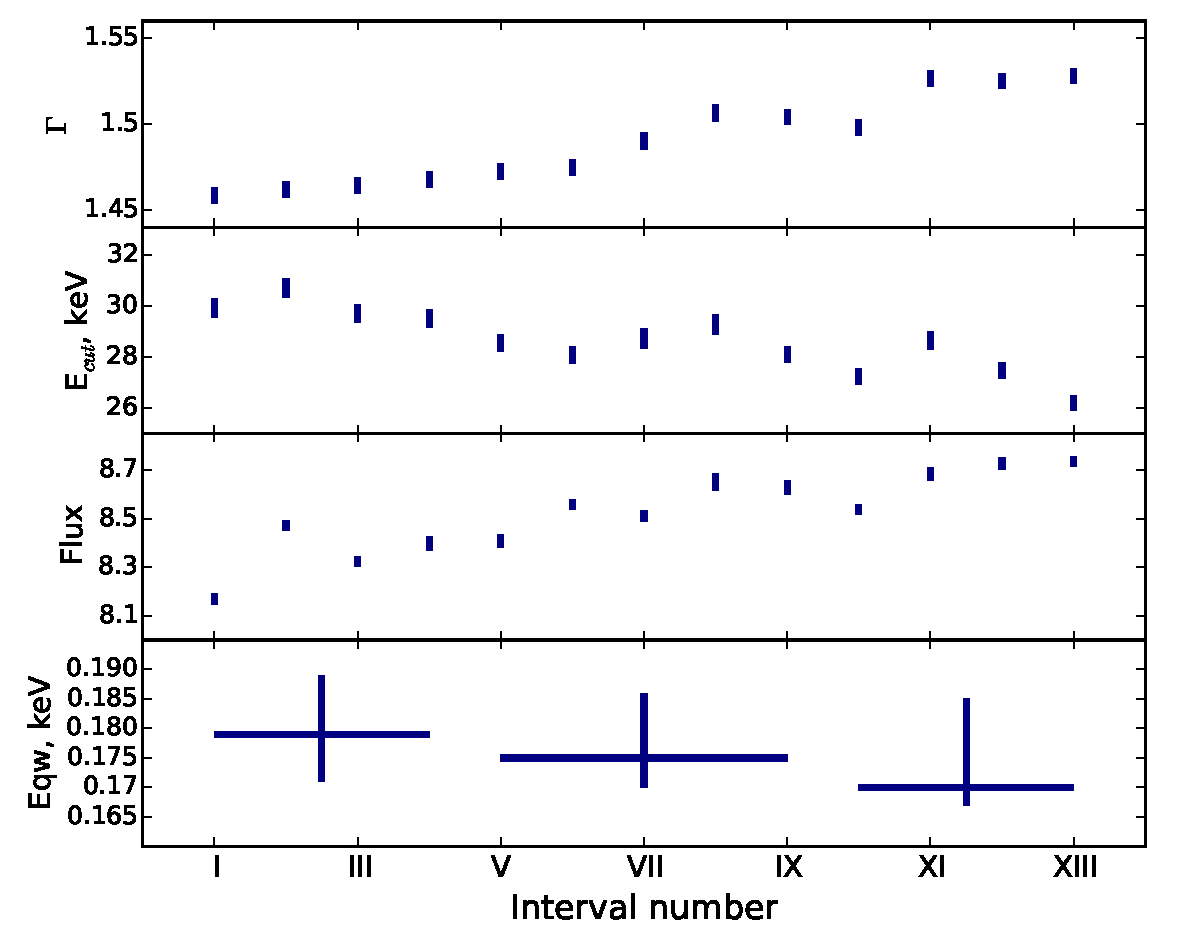
\includegraphics[width=\linewidth]{intspe_v04.eps}}
\caption{Parameters of continuum emission in intervals. From upper to lower: \texttt{xillver} powerlaw slope, cutoff energy,  flux in 3--60 keV band $\times$\, erg s$^{-1}$ cm$^{-2}$ and Fe $K\alpha$ line equivalent width obtained with \texttt{phabs$\times$(cutoffpl + gauss)} model (see sec.\ref{sec:continuum_evolution}).} 
\label{fig:intspe}
\end{figure}  

\begin{figure}
\centerline{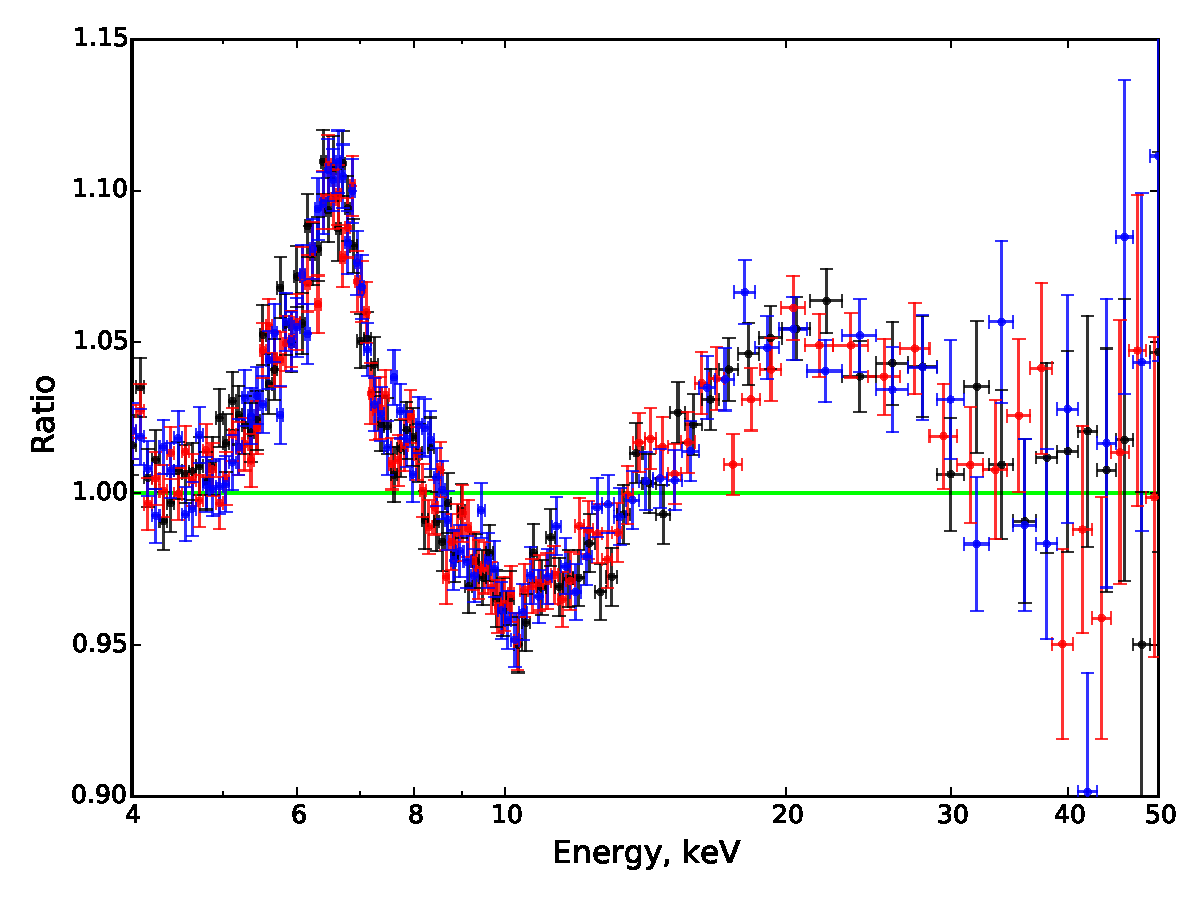
\includegraphics[width=\linewidth]{ratios_v01.pdf}}
\caption{Ratio of \nustar\, FMPA spectra to \texttt{phabs*cutoffpl} model. In black - data from intervals I-IV, in red from V-IX and in blue from X-XIII.} 
\label{fig:ratios}
\end{figure}  

            

\section{Timing analysis} 

Variability properties of different types of X-ray binary systems are usually described in terms of the power spectrum.
The power spectrum of the BHC systems in LHS/HIMS state can be described typically as a combination of a band-limited noise and one or few narrow Lorentzian functions, representing QPOs \citep[see, e.g.,][]{1972ApJ...174L..35T, 1990A&A...227L..33B, homan05}. 
Properties of these components and correlations between them, in principle, may be used to discriminate between different models of the formation of the X-ray emission in BHC systems. 
 
Although the power spectra analysis is by far the most popular method for the study of a physical properties of the accretion flow, more sophisticated methods, such as a coherence function or phase-lag were successfully applied as well. 
In particular, using a measured time-lag between the soft and hard emission, which has a complex behavior with the frequency, \citet{1999ApJ...517..355N} constrained a geometrical size of the accretion flow. 

In the following section we present results of the analysis of \grs\ timing properties and their evolution during the 2014 outburst.

\subsection{Power spectrum}

As it was mentioned above, we split {\it NuSTAR} observation of \grs\ into 13 continuous intervals separated with $\sim0.7$~hr gaps when the source was occulted by Earth. 
The continuous intervals have a duration about 3~ks (Table~\ref{tab:timing}).
Since {\it NuSTAR} detectors operate in the photon counting mode, data can be reduced to the lightcurve with the time resolution up to 2~$\mu$s.
For our analysis we extracted lightcurves with the 0.01~s temporal resolution in several energy bands (3--78, 3--5, 5--8, 8--15, 15--78~keV), which allows us to examine a frequency range of $\sim3\times10^{-3}$--$50$~Hz.
This frequency band usually contains low frequency QPOs and a broad band noise \citep{wijnands99}.
We produced a power spectrum for each interval of the {\it NuSTAR} observation using lightcurves in the 3--78~keV energy band.
All power spectra have a similar form: a plateau ($P(f)\propto const$) on the low frequencies, transforming at the frequency of $\approx0.1$~Hz in to the power law with the slope of $\rho\approx-1.6$..$-2.0$ and to the Poisson noise plateau at the frequencies above few Hz. 
A prominent QPO at the frequencies of 0.3--0.7~Hz and its second harmonic are present as well. 
Typical power spectrum (with subtracted Poisson noise, see text below) of a single interval is shown in Fig.~\ref{fig:qpo}.


In order to quantatively characterize properties of the broad band noise and QPOs we approximate each obtained power spectra with the following analytical function:
\begin{equation}
        \begin{aligned}
                P(f)  = & n (1 + (f/f_{\rm lb})^4)^{\alpha} + \\
                     &\frac{s_1}{(f - f_{\rm QPO})^2 + (f_{\rm QPO}/Q_{\rm m})^2} +\\
                        & \frac{s_2}{(f - 2f_{QPO})^2 + (2f_{\rm QPO}/Q_{\rm m})^2} + \\
                        & P_{\rm poiss}
\end{aligned}
        \label{eq:complex_fit}
\end{equation}
where $f_{\rm lb}$ is a broad noise break frequency; $f_{\rm QPO}$ and $Q_{\rm m}$ - centroid of the QPO and its quality correspondingly (quality of the QPO characterize the broadness of the QPO peak and therefore the stability of the Quasi Periodic process); $P_{\rm poiss}$ represents mean power of the variations caused by the counting statistics and dumped by the dead-time.
In this function first component represents plateau with the break, second two components describe QPO main harmonics and its overtone, last component represents Poisson noise.
We take that the quality of the second harmonic of QPO is equal to the QPO quality.
In following we will mention this models as standard.

In order to determine properly all parameters one have to know the shape and normalization of the Poission noise component, which depend on the countrate and dead-time and in principle can be described with analytical functions \citep[see, e.g.,][]{1994A&A...287...73V, 1995ApJ...449..930Z}.
{\it NuSTAR} detectors are subject to a non-paralyzing dead-time with the characteristic timescale of $\tau \approx 2.5$~ms \citep{2015ApJ...800..109B}.
In our case effects from dead-time already can be observed in power spectra at frequencies above 20~Hz.
\citet{2015ApJ...800..109B} noted that the {\it NuSTAR} dead-time has a complex dependence on the energy of registered photons, and therefore it is hard to create an analytical model for the power spectrum of Poisson noise. 
To avoid this problem they proposed to use a cross-spectrum (or shortly cospectrum) for analysis of {\it NuSTAR} data instead of the power spectrum. 
Authors define the cospectrum as a real part of the cross product of Fourier function of light-curves obtained from two {\it NuSTAR} detectors 
\begin{equation}
        \label{eq: ps_estimation}
        P(f) \approx <re(F_{\rm FPMA}^{*}(f)F_{\rm FPMB}(f))>
\end{equation}
where $P(f)$ is the estimation of the studied source intrinsic variability power spectrum, $F_{\rm FPMA[B]}$ is Fourier function of a light curve from FPMA[B] modules, asterisk stands for complex conjugation. 
This method is based on the following assumptions: signals produced by an observed source on two detectors are identical and have no time lag and therefore their Fourier functions are also identical and have zero phase shift; in contrast, signals independent for two detectors (like counting statistics) have random phase shifts.  
As a sequence for independent signals the average real part of the cross product tends to zero due to the random phase shift, i.e. Poisson noise is eliminated.

\citet{2017arXiv170909666H} shown that the cospectrum value in each frequency bin is distributed with the Laplace probability density function (PDF), if it is derived from two normally distributed random independent series \citep[see, e.q., eq.~14 in ][]{2017arXiv170909666H}:
\begin{equation}
        p(C_{j}|0, \sigma_x \sigma_y) = \frac{1}{\sigma_x \sigma_y} exp{\left(\frac{-|C_{j}|}{\sigma_x \sigma_y} \right)}
\end{equation}
where $C_{j}$ is the cospectrum of two {\it uncoherent} series measured in the $j$-th frequency channel and $\sigma_x$, $\sigma_y$  are second momenta of the initial normal distributions which were combined to produce Laplace distribution. 
These values ($\sigma_x$, $\sigma_y$) are equal to the square of the power spectra in corresponding frequency channel for each time series).
If signals used for the cospectrum estimation have identical power spectra then $\sigma_x = \sigma_y \approx |F_{\rm FPMA}|$.
We, therefore, see that to determine proper likelihood function which can be used to approximate cospectra with analytical functions, one still has to know Poisson noise level.
It is also worth noting, that source countrate and total countrate are usually slightly differs for two {\it NuSTAR} modules making amplitudes of counting-statistic and dead-time not equal.
Taking all this arguments into consideration we decided to use standard power spectrum analysis to estimate properties of the source intrinsic variability.

Since we used relatively large time binning (10 ms) to extract lightcurves from {\it NuSTAR} data and considered variability at frequencies below 10~Hz (where signal to noise ratio is sufficient), we assumed that the only effect from the dead-time is lowering of the constant Poisson noise level on the factor $(1 - 2\nu \tau_{\rm d})$, where $\nu$ is total count rate for detector and $\tau_{\rm d}$ is a dead time \citep{1994A&A...287...73V, 1995ApJ...449..930Z}. 
As the dead-time is not constant with the energy, we determined a modified Poisson level for each extracted data-set separately.


We did not consider any high frequency QPOs, since the typical HF QPO (centroid frequency 100-400~Hz, amplitude $\approx10$\% and quality $Q\approx2$--$10$) is indiscernible over the Poisson noise with the obtained count-rate and duration of the observation.


\begin{figure}
        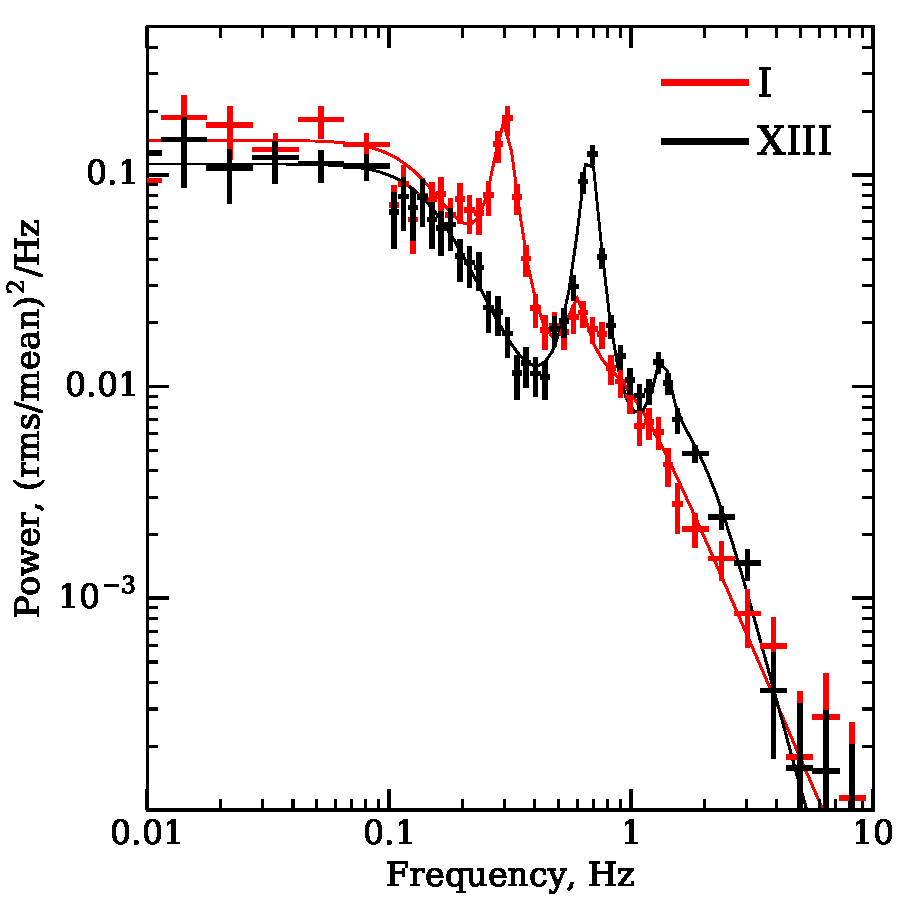
\includegraphics[width=\columnwidth]{qpo_centroid_evolution.pdf}
        \caption{Power spectrum of the \grs\ obtained with {\it NuSTAR} data at the beginning (red crosses) and at the end (black crosses) of the observation. Poisson noise is subtracted.}
        \label{fig:qpo}
\end{figure}

\begin{figure}
        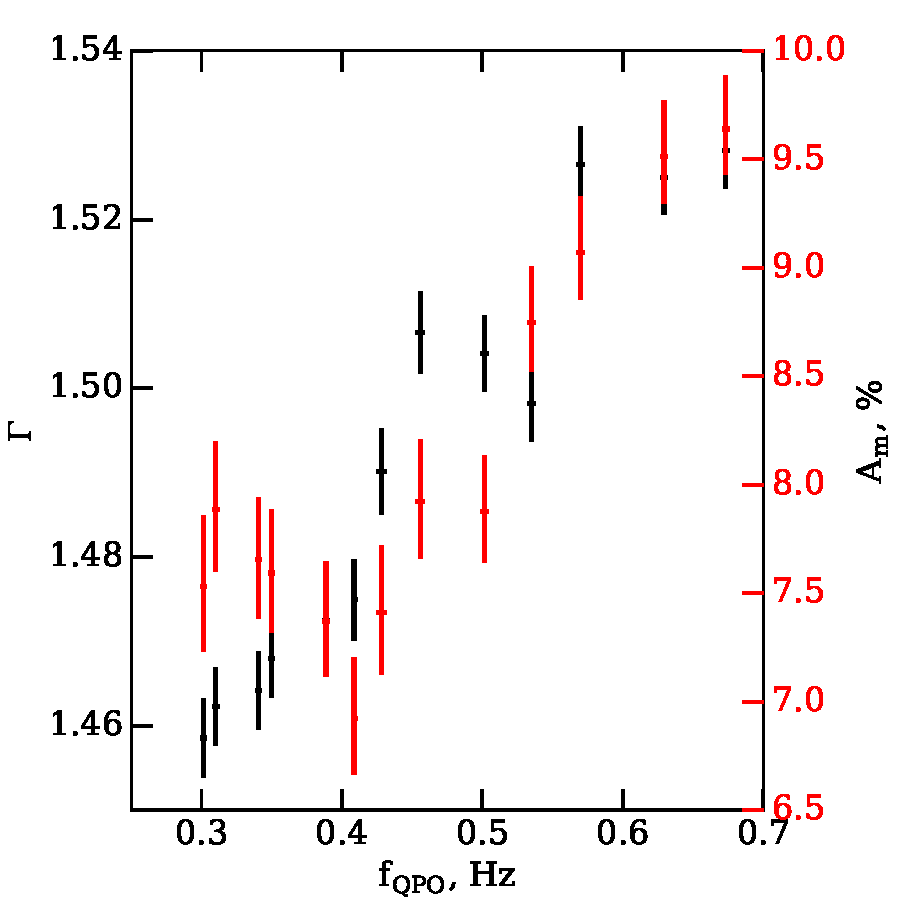
\includegraphics[width=\columnwidth]{QPO_correlation_graph.pdf}
        \caption{Observed dependence of the energy spectrum photon index (black crosses) and the QPO amplitude (red crosses) on the QPO centroid frequency}
        \label{fig:qpo_gamma}
\end{figure}


We found that the QPO frequency evolves with time (Table~\ref{tab:timing} and Fig.~\ref{fig:qpo}).
It correlates with the {\it NuSTAR} flux and photon index (see, Fig.~\ref{fig:qpo_gamma}), similar to many other black hole and neutron star binary systems \citep[see, e.g.,][]{2000ApJ...531..537S, vignarca03,2003A&A...407.1039P, fuerst16}.
The QPO amplitude remained stable during the first half of the observation, and started to grow in the second part.

\begin{table*}
\noindent
\centering
\caption{Evolution of the Fourier and energy spectrum properties through the {\it NuSTAR} observation in the 3--78~keV energy band.}
\label{tab:timing}
\centering
\begin{tabular}{|c|c|c|c|c|c|c|c|c|c|c|}
\hline\hline
Interval    & T$_{start}$,  & Expo,     & f$_{\rm br}$,                     & f$_{\rm QPO}$, & Q$_{\rm m}$,     & A$_{\rm m}$,  & A$_{\rm o}$,      & rms & $\Gamma$ & E$_{\rm cut}$, \\
            &  MJD          &  s        & $\times10^{-2}$, Hz               &  Hz            &   & \%            &  \%               &   \%       &          &  keV             \\
\hline
I           & 56742.68      & 3386      & $8.9_{-2.3}^{+2.2}$  & $0.30\pm0.01$ & $15_{-3}^{+5}$ & $7.5_{-1.0}^{+0.9}$ & $2.7_{-0.9}^{+0.8}$ & $26\pm1$ & $1.459\pm0.005$ & $29.9\pm0.4$ \\
II & 56742.75 & 3388 & $7.8_{-1.8}^{+2.0}$ & $0.31\pm0.01$ & $13\pm3$ & $7.9_{-0.9}^{+1.0}$ & $2.7_{-0.9}^{+0.8}$ & $26\pm1$ & $1.462\pm0.005$ & $30.7\pm0.4$ \\
III & 56742.82 & 3392 & $8.2_{-1.9}^{+2.4}$ & $0.34\pm0.01$ & $12_{-2}^{+3}$ & $7.7_{-0.8}^{+0.9}$ & $3.9_{-0.8}^{+0.9}$ & $26\pm1$ & $1.464\pm0.005$ & $29.7\pm0.4$ \\
IV & 56742.88 & 3389 & $8.3_{-1.8}^{+2.0}$ & $0.35\pm0.01$ & $15_{-3}^{+4}$ & $7.6\pm0.9$ & $3.2_{-0.8}^{+0.7}$ & $26\pm1$ & $1.468\pm0.005$ & $29.5_{-0.3}^{+0.4}$ \\
V & 56742.95 & 3389 & $6.9_{-1.4}^{+1.6}$ & $0.39\pm0.01$ & $13_{-3}^{+4}$ & $7.4\pm0.8$ & $4.3_{-0.9}^{+0.8}$ & $26\pm1$ & $1.473\pm0.005$ & $28.6\pm0.3$ \\
VI & 56743.02 & 3136 & $7.5_{-1.5}^{+1.9}$ & $0.41\pm0.01$ & $17_{-3}^{+5}$ & $6.9_{-0.8}^{+0.9}$ & $3.8_{-0.8}^{+0.7}$ & $26\pm1$ & $1.475\pm0.005$ & $28.1\pm0.3$ \\
VII & 56743.09 & 2771 & $9.7_{-2.2}^{+2.7}$ & $0.43\pm0.01$ & $12_{-2}^{+3}$ & $7.4\pm0.9$ & $3.6\pm0.9$ & $26_{-1}^{+2}$ & $1.500\pm0.005$ & $28.7\pm0.4$ \\
VIII & 56743.15 & 3387 & $5.8_{-1.5}^{+1.4}$ & $0.46\pm0.01$ & $11_{-2}^{+3}$ & $7.9\pm0.9$ & $4.2_{-0.8}^{+0.9}$ & $27\pm2$ & $1.507\pm0.005$ & $29.3\pm0.4$ \\
IX & 56743.22 & 3392 & $7.1_{-1.4}^{+1.6}$ & $0.50\pm0.01$ & $12_{-2}^{+4}$ & $7.9\pm0.8$ & $4.3\pm0.8$ & $26\pm1$ & $1.504\pm0.005$ & $28.1\pm0.3$ \\
X & 56743.29 & 3390 & $7.0_{-1.6}^{+1.7}$ & $0.53\pm0.01$ & $13_{-2}^{+3}$ & $8.7\pm0.7$ & $4.5_{-0.8}^{+0.7}$ & $25\pm1$ & $1.498\pm0.005$ & $27.2\pm0.3$ \\
XI & 56743.35 & 3382 & $(6.7\pm1.5)$ & $0.57\pm0.01$ & $13\pm3$ & $9.1_{-0.7}^{+0.8}$ & $4.0\pm0.8$ & $25\pm1$ & $1.527_{-0.005}^{+0.004}$ & $28.7\pm0.3$ \\
XII & 56743.42 & 3386 & $6.7_{-1.4}^{+1.8}$ & $0.63\pm0.01$ & $14_{-2}^{+3}$ & $9.5_{-0.7}^{+0.8}$ & $4.4\pm0.7$ & $26_{-1}^{+2}$ & $1.525\pm0.004$ & $27.5\pm0.3$ \\
XIII & 56743.49 & 3391 & $7.5_{-1.5}^{+1.7}$ & $0.67\pm0.01$ & $15\pm3$ & $9.6\pm0.7$ & $4.2\pm0.8$ & $25_{-1}^{+2}$ & $1.528\pm0.004$ & $26.2\pm0.3$ \\
\hline
\end{tabular}
\begin{flushleft}
        In Table $f_{\rm br}$ is broad band noise break frequency, $f_{\rm QPO}$ is the QPO centroid frequency, $Q_{\rm m}$ is QPO main harmonic quality (ratio of its centroid frequency to its width), $A_{\rm m}$ - total power in the QPO main harmonic in \% of mean countrate, $A_{\rm m}$ is total power in the QPO second harmonic in \% of mean countrate, rms - total amplitude of variations in the \% of mean countrate, $\Gamma$ - powerlaw photon index, $E_{\rm cut}$ - powerlaw cutoff energy. Parameters $\Gamma$ and $E_{\rm cut}$ were obtained from spectra of individual intervals with {\it xillver} model (see sec.\ref{sec:continuum_evolution}).
\end{flushleft}
\end{table*}


We also inspected power spectra in soft (3--5~keV) and hard (15--78~keV) energy bands and found that the QPO amplitude is smaller in the soft band, while amplitude of its harmonic is larger.
The ratio of the power in the QPO and its second harmonic for hard and soft energy bands is presented in Fig.~\ref{fig:qpo_ratio}.
\begin{figure}
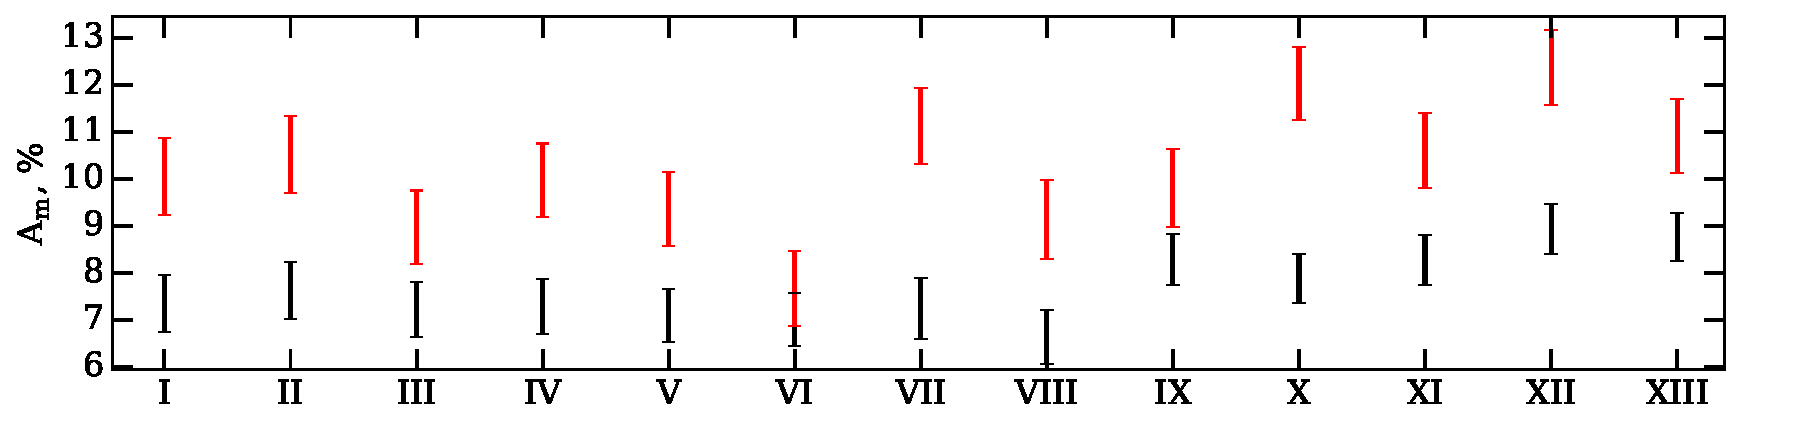
\includegraphics[width=\columnwidth]{Q_ampl2.pdf}
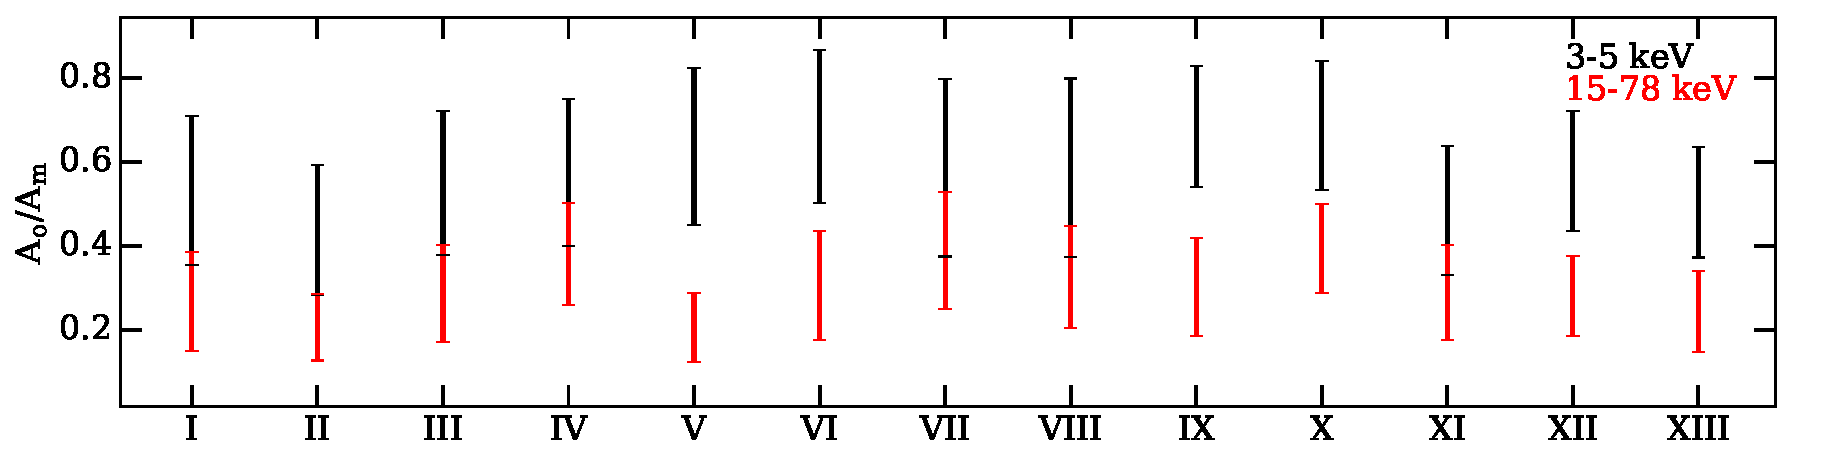
\includegraphics[width=\columnwidth]{QPO_and_harmonic_ratio_ylabel.pdf}
        \caption{On top panel: amplitude of the QPO harmonic in \% of mean countrate, on the bottom panel: ratio of the total power in the QPO and its second harmonic measured for the lightcurves obtained in 3--5~keV and 15--78~keV energy bands.}
        \label{fig:qpo_ratio}
\end{figure}
\citet{2015MNRAS.446.3516I} proposed that the ratio between the QPO first and other harmonics is determined by the particular pulse profile (stable in time with small distortions, which determine QPO quality) and derived such pulse profile in GRS~1915+105.
From the changing ratio between the QPO and its harmonics it follows that the pulse profile is changing with energy. 
Following \citet{2015MNRAS.446.3516I} we tried to extract QPO profile by segregating the coherent part (Fourier signal with conserving phase shift relative to the signal on the QPO frequency) between the QPO and its harmonics, however no significant coherence was detected above the noise level.
It indicates that the pulse profile was not stable during the observation, in contrast with the result obtained by \citet{2015MNRAS.446.3516I} for GRS~1915+105 with {\it RXTE} observatory data.

In some intervals QPO subharmonics (another peak like feature in the power spectrum), centered approximately at 1/2 of the QPO centroid frequency, is clearly observed in the cospectra (see examples on Fig.~\ref{fig:cospec_tracked}, red crosses) (namely I, II, IV, V, VI sets).
In order to detect QPO with the better significance we stacked several cospectra, frequency of each cospectrum was scaled in such a way to conserve QPO centroid at 0.3~Hz.
Obtained ``tracked'' cospectrum is presented on Fig.~\ref{fig:cospec_tracked}.
The subharmonics seems to roam around the 1/2 QPO frequency, therefore we were not able to obtain it with a large significance on the tracked cospectrum.


\begin{figure}
        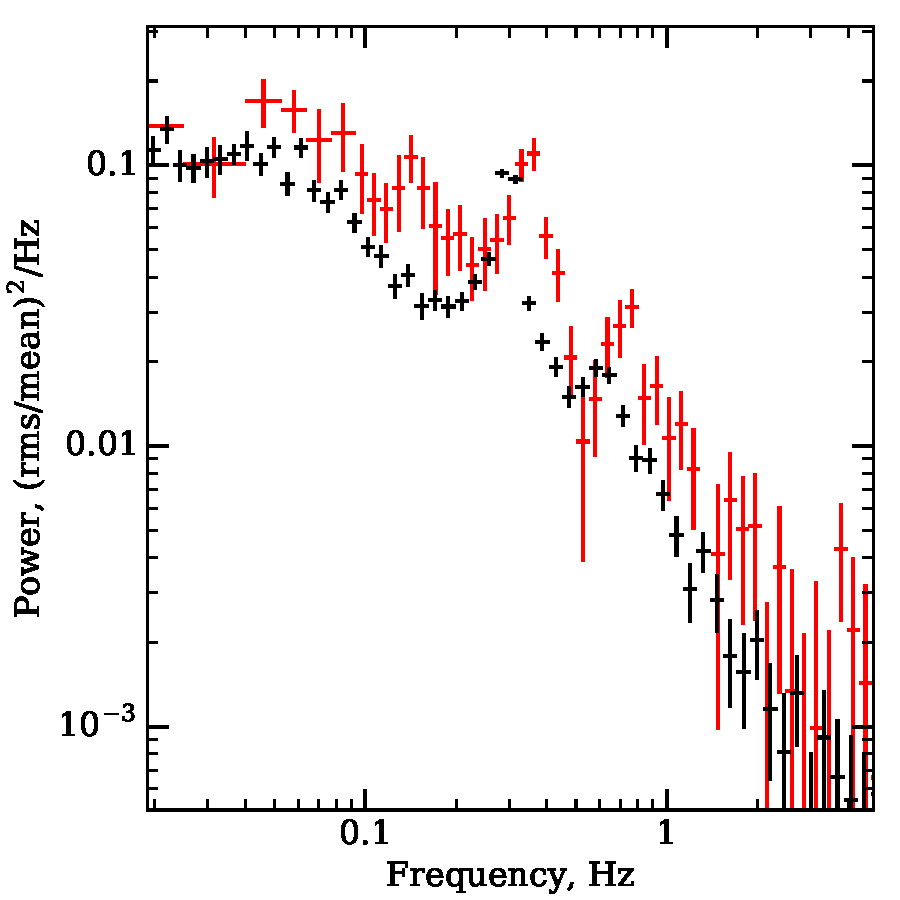
\includegraphics[width=\columnwidth]{subharmonics2.pdf}
        \caption{Cross-spectrum of the observations, obtained by scaling frequency to conserve QPO position.
        Black crosses obtained from the all intervals, while red crosses are from interval IV in which QPO subharmonics was most prominent.}
        \label{fig:cospec_tracked}
\end{figure}

It should be noted that the changes in the QPO centroid position during each interval may contribute to the measured quality factor $Q$ due to the relatively large QPO frequency changing speed $d{f}_{\rm QPO}/dt \approx 5.0$--$6.5\times10^{-6}$~Hz~s$^{-1}$ and relatively short time of separate intervals $\approx3000$~s.
Such movement of the QPO centroid frequency during the interval results in the measured quality $Q \approx 17$ even if its real value is much higher (QPO is almost periodical).
To check does this effect bring any distortions in our quality measurements we introduced another model to fit power spectra, which take in to account QPO centroid frequency movement. 
In this model we fitted simultaneously multiple power spectra obtained from the shorter intervals, amplitude and the QPO quality were taken to be equal for all power spectra, while for the QPO centroid frequency  linearly evolves with time.
Obtained quality factors are in good agreement with those obtained with more simple model, the median value $Q=14.3$.

\subsection{Coherence}

\defcitealias{1997ApJ...474L..43V}{VN97}
\citet{1997ApJ...474L..43V}(hereafter \citetalias{1997ApJ...474L..43V}) suggested to use a coherence between different energy bands in order to obtain an additional information from the source variability. 
The coherence measures the similarity between two signals and can be calculated with the following expression:
\begin{equation}
        C(f) = \frac{|<F_{\rm s}(f)^*F_{\rm h}(f)>|^2 - n^2}{P_{\rm s}(f) P_{\rm h}(f)}
    \label{eq:nowak_coh}
\end{equation}
where $F_{\rm h}(f)$ and $F_{\rm s}(f)$ are Fourier functions of the observed time series in hard and soft bands, correspondingly, $P_{\rm s}(f)$ and $P_{\rm h}(f)$ is estimation of their power density spectra (derived, for example, with the Equation~\ref{eq: ps_estimation}),  
$n^2$ - product of the power in the uncorrelated noise components divided by the number of used series (which mostly determined by Poisson statistics noise, see \citetalias{1997ApJ...474L..43V}). 
Since the coherence is estimated as a mean product of the Fourier functions it should be computed for the number of independent time series, therefore we separated each of the available uninterrupted time intervals on several shorter parts, 82~s long each.  


Different models of the XRBs variability generation suggest that signals in two energy bands can be partially independent, while the shape of the power spectra is conserved.
It appears that in many sources the coherence between soft and hard X-ray bands is close to unity \citep{1999ApJ...517..355N, wijnands99}, however there were also indications  on complex picture of the coherence in particular state of some systems \citep[dip in the coherence at 0.03~Hz frequency, observed in GRS1915+105, ][]{2003ApJ...584L..23J}, \citep[decreasing of the coherence between particular energy bandse in GX 339--4, ][]{1997ApJ...474L..43V}.
See also discussion in the \citetalias{1997ApJ...474L..43V} for the theoretical prediction on the coherence for different models.

Following \citetalias{1997ApJ...474L..43V}, we estimated the coherence of \grs\ light-curves obtained in different soft and hard energy bands. 
Since we use {\it NuSTAR} data (covering 3--79~keV energy band) we adopted following energy bands for our analysis: 3--5~keV, 5--8~keV, 8--15~keV and 15--78~keV.
This partition of the {\it NuSTAR} energy band pursues the following idea: the energy spectrum of \grs\ can be described with two major components - powerlaw continuum and reflection features i.e. the fluorescent Fe K$\alpha$ line and the Compton hump.
In the 5--8~kev band there is a contribution of the prominent Fe K$\alpha$ line, with the equivalent width of 0.2~keV it provides about 5\% of the flux in this band.
In the 8--15~keV energy band we expect only the power law component to be present.
Compton hump, another reflection feature, is confined in the 15--78~kev energy band. 

As it was mentioned above the {\it NuSTAR} detectors have a complex dead-time depending on the energy, the coherence computed from one detector is subject to the dead-time cross-talk effects (i.e. capturing of the photon in particular energy band prevents registration of any next photon arriving during the dead-time, see e.g. \citet{2015MNRAS.451.4253R}). 
Such cross-talk makes more coherent random processes, independent in different energy channels.
In order to eliminate these effects in coherence estimation we follow the recipe suggested by \citet{2015ApJ...800..109B} for the cospectrum estimation. 
As explained in \citet{2015ApJ...800..109B} we can take advantage of the presence of two detectors modules, signals from which are processed independently. 
That means that the photon registered by one of the modules do not prevent registration of the photon arriving during the dead-time in another module. 
Therefore, for the numenator in Eq~\ref{eq:nowak_coh} (cross product of the Fourier functions of the light-curves obtained in different energy bands) we use light-curves obtained from different modules - e.g. lightcurve obtained in soft band on FPMA with one obtained in hard band on FPMB and vice versa.

To obtain proper estimation on the coherence it is also important to have the correct estimation of the intrinsic variability power spectrum (denumenator in Eq.~\ref{eq:nowak_coh}).
We use in this work model independent approach, with the cospectrum used for the power spectrum estimation (another approach would be to use Poisson noise subtracted power spectrum or analytical function fitted to the power spectrum in the previous section).

The $n^2$ component was computed as it is suggested by \citetalias{1997ApJ...474L..43V}. 
We estimated Poisson noise level as a mean power in the 5--15~Hz range, in this frequency band Poisson noise dominating over the source intrinsic variability, while its shape yet not affected by the dead-time effects (the spectrum is flat below 15~Hz).

By using the cospectrum for the intrinsic variability power spectrum estimation we introduce one drawback. 
As was discussed in the previous section cospectrum can be described with Laplace statistics, which have non-zero probability density in the vicinity of zero and positive mean value.
Therefore, if insufficient number of samples are used to calculate the mean of the cospectrum than the enormous statistical errors would be introduced in the coherence (since the cospectrum is used in the denominator in its estimation).
The number of the samples is limited by the total duration of the observation and the condition that the shape of the cospectrum should not changing significantly in used samples (otherwise artificial dispersion would be introduced in the cospectrum distribution).
The last criterion appears to be more strict one, since the QPO and break frequencies are changed by a factor of two during the observation.
In order to increase statistical significance of the estimated cospectrum we use the following property found to be inherent for the XRBs intrinsic variability. 
\citet{wijnands99} shown that primary features of the power spectrum of the XRBs in low-hard and high intermediate states are evolving simultaneously, i.e. the break frequency of the flat top broad band noise and the QPO centroid frequency are connected with the relation $f_{\rm b} \approx 0.3 f_{\rm QPO}$.
Bearing in mind this property of the power spectrum and small scatter in the $f_{\rm b}/f_{\rm QPO}$ in our data, we stacked all 13 separate intervals of the observation, scaling their frequencies to preserve QPO position. 
We assumed that the coherence in each tracked frequency channel is preserved along the observation and scaled in the similar way.

\begin{figure}
    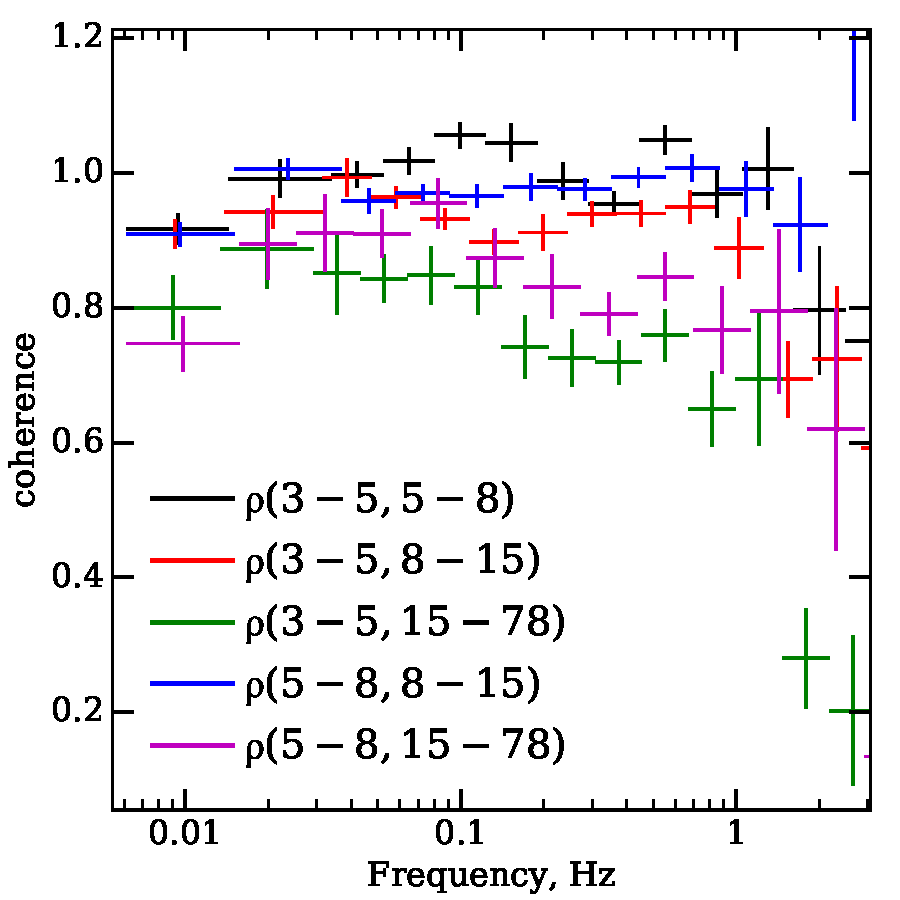
\includegraphics[width=\columnwidth]{coherence_5.pdf}
    \caption{Coherence between lightcurves extracted in different energy bands: black, red, green, blue and magenta are for (3--5, 5--8), (3--5, 8--15), (3--5, 15--78), (5--8, 8--15) and (5--8, 15--78) correspondingly.}
    \label{fig:coherence}
\end{figure}

The coherence between hard and soft energy bands at frequencies up to $\sim3$~Hz is presented in Fig.~\ref{fig:coherence}. 
We found that the coherence in the adjacent energy bands is close to unity, with mean values in 0.01--1~Hz frequency band being $1.0\pm0.05$.
However for the 3--5 and 15--78~keV energy bands the coherence is significantly lower (Fig.~\ref{fig:coherence}). 
It is on the nearly constant level of $\approx0.85$ in the (0.005--0.1)~Hz frequency band and drops down above this frequency.
Analogous behavior was observed in GX 339--4 \citepalias{1997ApJ...474L..43V}, in this work authors also discussed possible mechanisms which could lead to such loss of coherence between different energy bands. 
Two main possibilities discussed by \citetalias{1997ApJ...474L..43V} were a) nonlinear transfer function between soft and hard bands and b) contribution of several coherent (within two energy bands) but independent processes in each energy band.
Both this scenarios can take place along with the model of propagating fluctuations, considered in this work.
First one would have require nonlinear process in the formation of the soft and hard emission, and the second require spatial separation of the soft and hard emission regions along the accretion flow. 


\begin{figure*}
        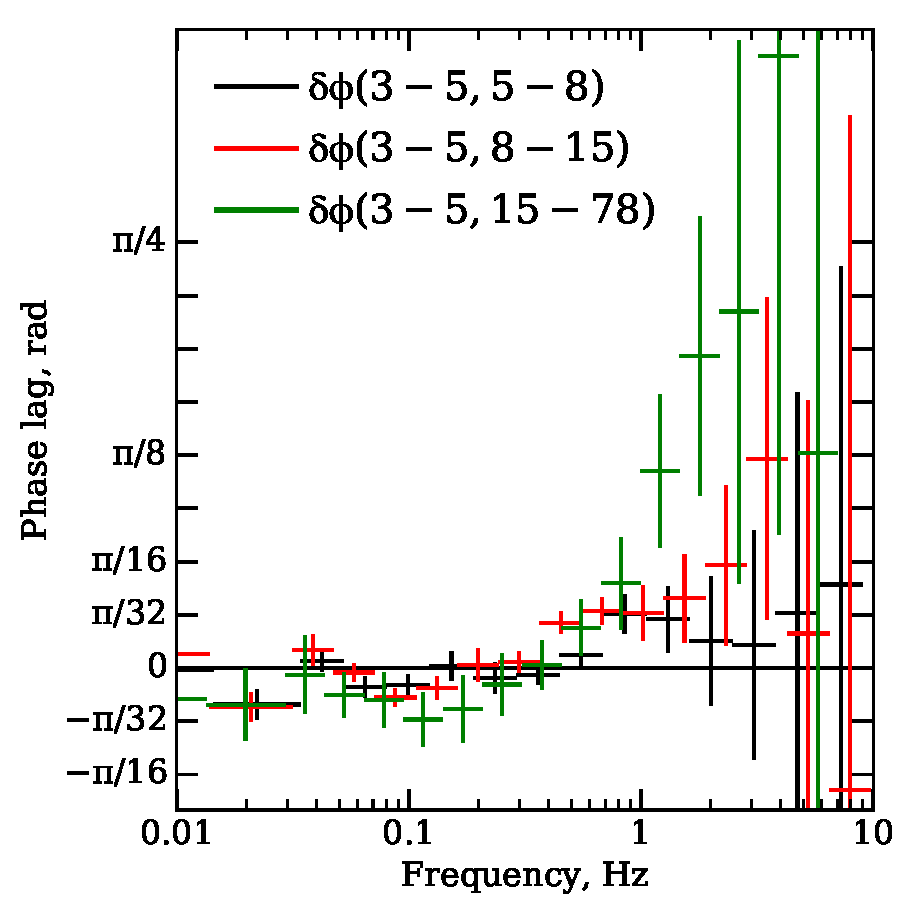
\includegraphics[width=0.99\columnwidth]{phase_lag_linear_fixed_fqpo.pdf}
        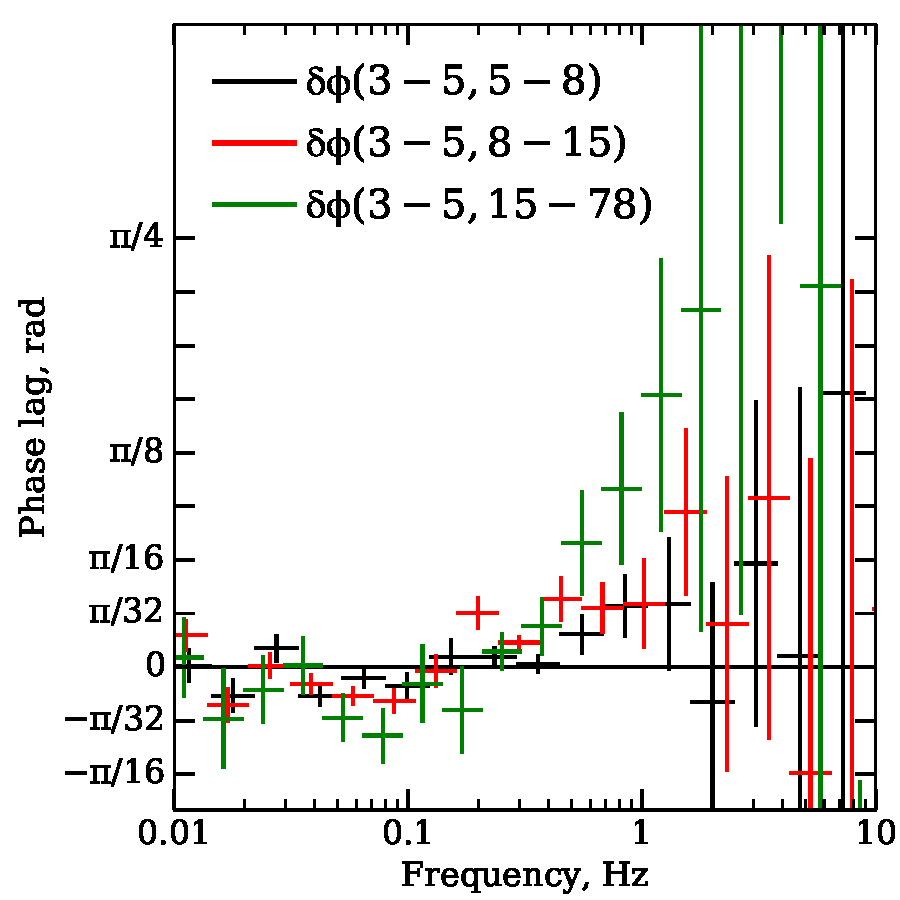
\includegraphics[width=0.99\columnwidth]{phase_lag_linear_y_traced_qpo.pdf}
        \caption{Phase lag between the soft (3--5~keV) and hard (5--8; 8--15; 15--78~keV) energy bands in \grs. 
        On the left panel - phase lag spectrum obtained from {\it NuSTAR} observations by stacking all data, on the right panel same spectrum with tracked frequency (frequency for each separate light-curve segment was scaled such a way to conserve QPO centroid at 0.3~Hz).}
        \label{fig:phase_lag}
\end{figure*}

\begin{table*}
\noindent
\centering
\caption{QPOs detected in \swiftx\, observations}
\label{tab:xrtqpo}
\centering
\begin{tabular}{|c|c|c|c|c|c|}
\hline\hline
Segment &$t_{mean}$                   & $f_{QPO}$, Hz & QPO $rms$, \% & Total $rms$, \% & Type\\
                &   days from $\tau_{0}$     &                           &                           &                            &\\
\hline
03  &17.9&  $0.37\pm0.01$            & $9\pm2$       & $28\pm3$        & C\\
04  &21.9&  $2.17\pm0.03$            & $8_{-2}^{+1}$ & $14_{-1}^{+2}$  & B\\
05  &26.8&  $1.67_{-0.04}^{+0.03}$   & $8\pm1$       & $17_{-3}^{+6}$  & B\\ 
06  &31.8&  $5.05\pm0.09$            & $4_{-1}^{+2}$ & $11_{-1}^{+2}$  & B\\
07  &36.0&  $2.52_{-0.08}^{+0.07}$   & $7_{-2}^{+1}$ & $15_{-2}^{+3}$  & B\\ 
08  &39.8&  $5.10_{-0.14}^{+0.16}$   & $5\pm1$       & $12_{-2}^{+3}$  & B\\
09  &46.6&  $2.17_{-0.04}^{+0.02}$   & $7_{-1}^{+2}$ & $17_{-3}^{+4}$  & B\\
\hline
\end{tabular}
\end{table*}

\subsection{Phase lags}

        The phase lags in different BHC system was being investigated by many authors \citep[see, e.g.][]{2003A&A...407..335M, 2006A&A...449..703R, 2011A&A...533A...8B, 2011MNRAS.415..292M, 2013MNRAS.435.2132M, 2017MNRAS.471.1475D}.
It was found that for stellar mass black holes the phase lag in the frequency range occupied by the flat-top noise and LF QPOs is usually hard and can be described with the power law $\Delta \phi /(2\pi f) = \Delta \tau \propto f^{-0.7}$ \citep{1989Natur.342..773M, 1999ApJ...517..355N} with positive or negative pikes at the QPO and its harmonics frequencies. 
\citet{1989Natur.342..773M} tried to explain observed lags with the clumpy flow model, which previously was used to explain an observed shape of the flat-top noise Fourier spectrum.
\citet{1999ApJ...515..726N} considered two models, promising to explain observed hard lags and their dependence on frequency - i.e. phase lags are formed due to Comptonization in the extended corona or they formed due to the propagation of the perturbations in the advection flow.  
They found that it is hard to explain observed phase lags with both models, with first demanding very extended corona ($\sim150 R_{\rm g}$) and second - very slow matter propagation speed in it.
Later \citet{2001MNRAS.327..799K} considered their result and, on the basis on the amplitude and energy dependence of the hard lag, derived that it can not be caused by the reverberation and is most preferably due to the perturbation propagation in the corona on the viscous time scales \citep[see also][on simulations results]{2006MNRAS.367..801A}.
It is worth mentioning, that proposed models are generally can explain hard lags but fail to explain soft lags, which were later found in many sources both on low and high frequencies (below and above flat-top noise break frequency) to mention a few \citep[][]{2010MNRAS.407.2166G, 2012MNRAS.427.2985C, 2017MNRAS.465.1926Y, 2017MNRAS.464.2643V}.
However, it was demonstrated that the soft lags are possible in the propagation fluctuation model if outward movement of the disk surface density perturbations due to viscous evolution are also considered \citep{2017arXiv170707578M}.  

\citet{2017ApJ...845..143Z} shown that in GX~339-4 BHC the phase lag at the QPO frequency and its second harmonic evolves with its frequency. 
\citet{2018MNRAS.473.4644R} found that the mean time lag strongly correlates with photon index of power law continuum, with the time lag increasing with decreasing hardness. 
They proposed, that observed behavior can be explained with the Comptonization of soft photons by energetic electrons in a jet.
\citet{2017MNRAS.464.2643V} found that the sign and amplitude of the phase lag at the QPO frequency depends on a system inclination.

From the definition of the coherence (see eq.~\ref{eq:nowak_coh}) it follows that signals have roughly constant phase shifts between their Fourier functions in each frequency bin where they are coherent. 
Following \citetalias{1997ApJ...474L..43V} to estimate the phase lags one have to calculate mean of the product of the Fourier function obtained in one energy band to the conjugated Fourier function estimated in second energy band, the phase of the obtained complex value would be the phase lag. 
\begin{equation}
      \delta \phi(f) = \arctan{\left(\frac{Im(<F_{\rm s}(f) F_{\rm h}^{*}(f)>)}{Re(<F_{\rm s}(f) F_{\rm h}^{*}(f)>)}\right)}
\end{equation}
Where $Im$ and $Re$ are stated for the imaginary and real part of the complex value correspondingly and $\delta \phi(f)$ is the frequency dependent phase lag. 
For the uncertainty estimation we used approach proposed by \citet{2014A&ARv..22...72U}, therefore $\Delta\delta\phi \approx \arctan{(\Delta C(f)/C(f))}$, where $C(f)$ - estimation of the coherence, and $\Delta C(f)$ is the coherence uncertainty estimation.

The phase lags observed for different systems had features, which correlated with the power spectrum and those which had not obvious counterpart in it. 
Therefore, bearing in mind property of the linear evolution of all frequencies of the power spectra discussed in previous section, we computed the phase lag spectrum with two approaches - with and without the QPO centroid frequency tracing (see right and left panels of Fig.\ref{fig:phase_lag}, correspondingly).
Obtained phase lags appears to be surprisingly similar, however those calculated with the traced QPO frequency are seem to have larger amplitude on the lower frequencies, which may indicate that phase lags are indeed evolves in a similar way with the power spectrum. 
It appears that in the 0.1--3~Hz frequency band positive (hard) lag is present while at frequencies below 0.1~Hz there are indication of the negative (soft) lag.
Observed phase lag corresponds to the delay times between soft and hard photons $\sim0.1$~s for frequencies above 0.1 Hz and $-0.1$..$-1$~s for frequencies below 0.1 Hz.
Unfortunately, due to insufficient signal to noise ratio, we can not determine, are there any specific features present at the QPO or its second harmonic centroid frequencies.    

\begin{figure}
    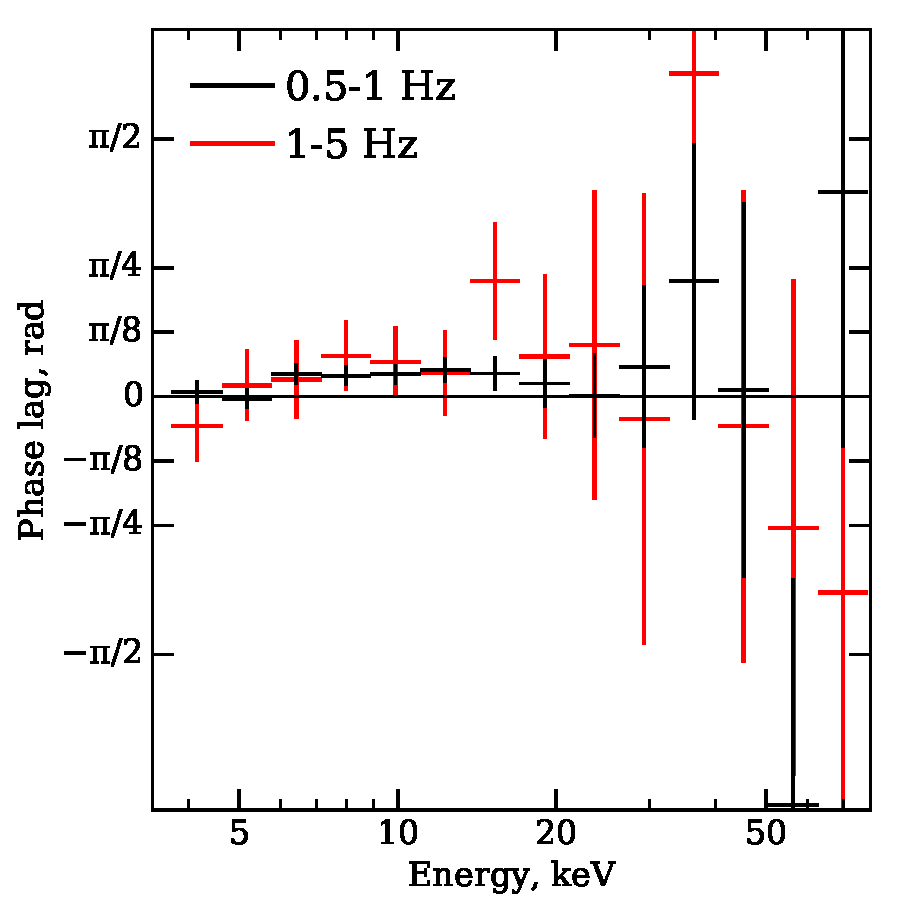
\includegraphics[width=\columnwidth]{phase_lag_en_dependence_2.pdf}
    \caption{Dependence of the phase-lag on energy calculated for the 0.5--1~Hz and 1--5~Hz frequency bands. All phase-lags are calculated relative to the softest energy band (3--3.72~keV).}
    \label{fig:ple}
\end{figure}

We also investigated phase-lag energy dependence for two frequency bands where they are most prominent (0.5--1~Hz and 1--5~Hz). 
We separate {\it NuSTAR} energy band on 15 logarithmically scaled bins and compute mean phase lag between the light curve in the first bin (3--3.72~keV) and all successive bins.
Obtained phase-lag--energy dependencies are presented in Fig.~\ref{fig:ple}.
While positive (hard) phase lag is observed for both frequency bands on energies above $\sim5$~keV, it does not changing significantly with energy. 
With the {\it RXTE} observatory data \citet{2001MNRAS.327..799K} found logarithmic growth of the phase-lag with energy, however, obtained in our data signal to noise ratio does not allow to robustly derive such a trend. 


\subsection{\swiftx\, observations}
We performed search for LF QPOs in first dozen of \swiftx\ observations of the \grs. 
QPO is clearly detected in observations 3 to 9, with frequency varying from 0.37 Hz (during simultaneous observation with \nustar, see Fig.~\ref{fig:nust_lc}) up to 5.1 Hz (see Tab.~\ref{tab:xrtqpo}). Last detection of QPO happened right before the onset of a strong flaring, at $\tau_{0}+46.6$. 

We used the shape of power spectra in order to classify QPOs as belonging to type C or B \citep{casella05}. 
In all observations except for the observation 03, low frequency parts of power spectra can be described with weak red noise, which typically accompanies type-B QPOs.
In order to reinforce classification we calculated $rms$ for each detected QPO, along with total $rms$ over 0.01--20 Hz band. 
Obtained $rms_{total}$ are significantly lower for observations 04..09 than for 03. 
We, therefore, conclude that in observations 04..09 type-B QPOs were observed with frequencies ranging from $\sim$2~Hz to 5~Hz.
It follows, that four days after the \nustar\ observation, the source already had transitioned from HIMS to SIMS and resided in this state until 09 \swiftx\ observation. 



\section{Discussion and conclusions}
We had studied the spectro-timing evolution of \grs\, during its hard-intermediate state. Using \nustar\, data we found a prominent type-C LF QPO in its power spectrum, with monotonically growing frequency. As its frequency increases from 0.3 to 0.7 Hz spectrum became softer: the power law index grows from 1.46 to 1.53 and cut-off energy decreases from 30 to 26 keV. Taking the advantage of the presence of the broad Fe K$\alpha$ emission line, which is usually thought to originate due to the reflection from the cold accretion disk, following the analysis performed earlier by \citet{miller15_nust}, we used {\texttt relxilllp} spectral model in order to estimate the accretion disk inner radius. Although the quality of the data prevented us from measuring a movement of the inner disk boundary throughout the observation, from the average broadband energy spectrum we found that the accretion disk is truncated at the radius smaller than 9 $GM/c^{2}$ (90\% confidence limit) which is in agreement with an estimates by \citet{miller15_nust}. 

We performed extensive timing analysis.  Power spectra is typical for HIMS and consist of the broadband noise and fundamental QPO, the second harmonic of the QPO is also seen. 
During several intervals from first half of the observation subharmonic was also observed. 
In all 13 intervals second QPO harmonic is more prominent in soft band (3--5 keV), with the ratio of its amplitude to that of 
fundamental QPO being $0.565\pm0.02$ in 3--5 keV band versus $0.275\pm0.02$ in 15--78 keV. 
Amplitude of fundamental QPO peak correlates with QPO  frequency and, consequently, with properties of energy spectrum (see, Fig.~\ref{fig:qpo_gamma}).
Measured velocity of the QPO drift is found to be $\approx6.0\times10^{-6}$~Hz~s$^{-1}$.

Coherence measured between the adjacent energy bands in 0.01-1 Hz was found to be nearly unity, while for the softest used energy band (3--5~keV) and the hardest energy band (15--78~keV) coherence turned out to be lower, with plateau breaking at 0.1~Hz . 
In the frame of the propagating fluctuations model it can be explained with the nonlinear process of the formation of soft and hard emission or with the separation of zones producing soft and hard emission along the accretion flow.

Time lag, corresponding to the phase lag found to be of order of $+0.1$~s (hard) in the 0.1--3~Hz frequency range and $-1$..$-0.1$~s (soft) below 0.1~Hz.
\citet{2017MNRAS.464.2643V} shown that the sign of the phase lag at the type-C QPO centroid frequency depends on a system inclination, however this difference is explicit only when the QPO centroid frequency is above $\sim3$~Hz, therefore we were not able to restrict \grs\ system inclination.
We found very small dependence of the phase-lag with the energy.
At the frequencies above 0.5~Hz the phase lag of the harder emission relative to the most soft {\it NuSTAR} channels grows up to $\approx \pi/16$ at the energies above $\approx7$~keV and stays relatively constant above it.

We searched for similar QPO in \swiftx\ observations of \grs\ performed after \nustar\, exposure and found that all other detected QPOs are probably of type B, thus the source transitioned to soft-intermediate state few days after \nustar\ observation.


\begin{figure}
        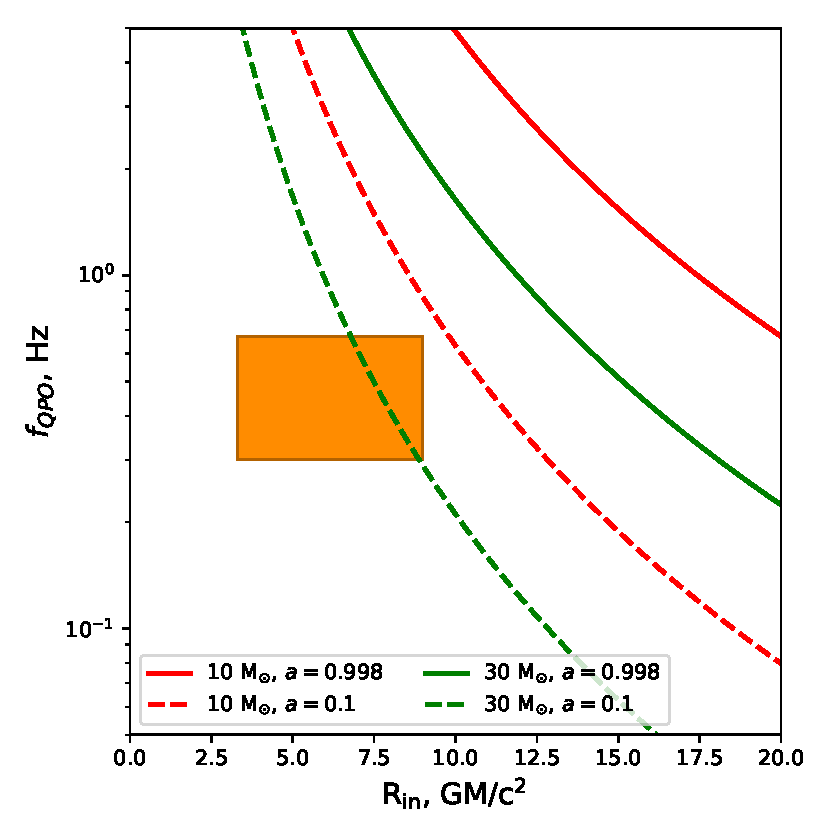
\includegraphics[width=\columnwidth]{qpoconstr_v04.pdf}
        \caption{Expected QPO frequency for a black hole of a given mass and spin versus the disk inner radius from \protect\cite{ingram14}. The orange square represents region bounded by observed QPO freuencies and measured disk inner radius.}
        \label{fig:qpoconstr}
\end{figure}


The Type-C QPO are believed to be caused by Lense-Thirring precession of the inner part of the accretion disk and, therefore, is strongly dependent on the truncation radius.
We used the combination of estimated disk inner radius and observed QPO frequencies in order to assess black hole mass, using the Lense-Thirring precession model of QPO origin \citep{ingram09}.
Following \citet{ingram14} we calculated nodal frequencies (which is though to correspond to the QPO fundamental frequency) versus the disk inner radius for two values of the black hole mass (10$M_{\odot}$ and 30$M_{\odot}$) and two values of the spin - $a=0.1$ and $a=0.998$ (maximally rotating). 
As it can be seen from Fig.~\ref{fig:qpoconstr} observations are incompatible with the black hole mass 10$M_{\odot}$ and barely agrees with the slowly rotating massive (30$M_{\odot}$) black hole. 
This results, along with the measurements by \cite{fuerst16_gx339, mereminskiy18_maxi}, indicates that there are some tensions between the predictions of RPM and the truncation radii inferred from the spectral fitting. It is also worth noting that the observed QPO changed in frequency by a factor $\approx2.5$, while no drastic changes were observed in the spectrum. 


\section*{Acknowledgments}
The work was supported by the Russian Science Foundation (grant no. 14-12-01287). 
We thank E.M. Churazov for fruitful discussions and important suggestions. 
We are grateful for T.Dauser and J.Gracia for their help with {\em relxill} model. 
This research has made use of data obtained through the High Energy Astrophysics Science Archive Research Center Online Service, provided by the NASA/Goddard Space Flight Center.
This work made use of data supplied by the UK Swift Science Data Centre at the University of Leicester.

%--------------------------------------------------------------------------------
\bibliographystyle{mnras}
\bibliography{author_en.bib,coherence.bib}
\bsp	
\label{lastpage}
\end{document}

